\documentclass{article}
\usepackage{graphicx} % Required for inserting images
\usepackage{amsmath}
\usepackage{caption}
\usepackage{amssymb}
\usepackage{array} % for tables
\usepackage{amsfonts}
\usepackage{tabularx}
\usepackage{geometry} % for tables and graphs 
\usepackage{hyperref}
\usepackage{float}
\usepackage{pgfplots} % for graphs in line
\usepackage{longtable}

\geometry{a4paper, margin=1in}
\pgfplotsset{compat=1.18}

% SECTIONS correspond to topics as covered in class
% MWG/JR chapters are written under the topic for reference
% notes re: important information included
% formulas and summary at the end of each section
% inclusion of PROBLEMS (from problem set / practices) that we may see 

\begin{document}

% Title Page
\begin{titlepage}
    \centering
    \vspace*{1in} % Vertical space at the top of the page
    {\LARGE \textbf{Microeconomics (ECON204A)}} \\[0.5cm]
    {\LARGE Allegra Saggese} \\ [.5cm]
    {\large 2024-25 UCSC Economics PhD} \\ [1.5 cm]
    {\large Fall 2024} \\[.25cm]
    {\large Natalia Lazatti} \\[1cm]
    \includegraphics[width=0.4\textwidth]{images/images.jpg} % Optional: include an image
    \vfill
    \end{titlepage}

% TOC
\clearpage
\pagestyle{empty} % ensures no headers on this page
\noindent \textbf{Last updated: \today} 
\vspace{0.5cm} % Adjust space before the TOC
\tableofcontents
\clearpage % next page
\pagestyle{plain} %remove headers




%%%%%%%%%%%%%%%% CONSUMER THEORY - WEEK 1 %%%%%%%%%%%%%%%%%
\section{Consumer Theory}
\subsubsection*{(MWG: 1, 3A-C, JR: 1.1-1.2)}

\subsection{Consumer Choice} % giving definitions / intuition

\begin{itemize}
    \item \textbf{Consumption set (choice set):}  $X$ is a set of alternatives or complete consumption plans (universe of alternative choices possible possible by consumer)
    \begin{itemize}
        \item \textbf{Consumption bundle} is $x$ where $x \in X$ (vector of $x_{1}, x_{2}, \ldots, x_{n}$ where $n$ is the number of total goods in that bundle).
        \item Properties of a consumption set: $X \subset \mathbb{R}^{n}$, $X$ is closed and convex. The null set is always in the set, $0 \in X$.
    \end{itemize}
    
    \item \textbf{Feasible set:} $B = \{ \text{all conceivable and obtainable consumption plans} \} \subseteq X$ regarding the accessing for any constraints. Where $B \subseteq X$.

    \item \textbf{Preference relation}: Specifies consumer's preference ability across choices, consistently or inconsistently. The preference relation is a binary relation on $X$, allowing for the comparison of alternatives $x, x' \in X$
    \begin{itemize}
        \item We can assume strict preferences $x_{1} \succ x_{2}$, if and only if $x_{1} \succeq x_{2}$ holds, and $x_{2} \succeq x_{1}$ does not hold. This means that $x_{2}$ can never be as good as $x_{1}$. If $x_{1} \succeq x_{2}$ and $x_{2} \succeq x_{1}$, then the relationship is indifference.
        \item These relations can be thought of as partitions in the consumption set, given the strict relationships ($x_{1} \succ x_{2}$, $x_{2} \succ x_{1}$, $x_{1} \sim x_{2}$) are mutually exclusive. 
    \end{itemize}
    
    \item \textbf{Behavioral assumption:} Identifies the objectives in a consuming choice (i.e. consumer seeks to find and select the alternative that is best in terms of preference or taste). 

% important! - axioms provide intuition, apply to all structures of bundles and goods, and used to determine optimal condition / outcomes of the model 
    \item \textbf{The axioms of consumer choice}: Gives math to the fundamental aspects of consumer behavior/attitudes, the consumer \textit{can} choose; therefore choices are consistent. Properties (axioms) of consumer theory allow us to make certain assumptions about the preferences made, which allow for evaluation of choice implications. \ref{tab:axioms_table}
    \begin{enumerate}
        \item \textbf{Completeness:} for all $x^{1}$ and $x^{2}$ $\in X$ either $x^{1} \succeq x_{2}$ or $x^{1} \preceq x_{2}$. This means consumers can actually compare bundles, they discriminate between two goods and make a decision based on the comparison. 
        \item \textbf{Transitivity:} For any three elements $x_{1}, x_{2}, x_{3}$, if $x^{1} \preceq x_{2}$ and $x^{2} \preceq x_{3}$ then $x^{1} \preceq x_{3}$. This demonstrates that consumer choices are consistent. 
        \item \textbf{Continuity:} for all $x \in \mathbb{R^{n}_{+}}$ at least as good ($\succeq$) and no better than ($\preceq$) are closed in $\mathbb{R^{n}_{+}}$. To note, they are closed where the complement is open in the domain. This guarantees that sudden preference reversals cannot occur. 
        \begin{itemize}
            \item Upper and lower contour sets are closed (so the set includes their boundaries)
            \item But continuity does not always imply differentiability, although this can be useful. \textit{The case of Leontif preferences where $x^1 \succeq x^2$ if and only if $\min \{ x^1_1, x^2_1 \} \geq \min \{ x^1_2, x^2_2 \}$ indicating there is a kink where $x_1=x_2$}
            \item If preferences have a utility representation, then the preferences are homothetic if and only if the utility is homogenous degree one: $u(\alpha*x) = \alpha*u(x)$ for all $\alpha$
        \end{itemize}
        \item \textbf{Local nonsatiation:} $\forall x^0 \in \mathbb{R}^n, \forall \epsilon > 0, \exists \textit{ x} \in B_\epsilon(x^0) \cap \mathbb{R}^n \text{ such that } x > x^0$. This rules out any "zones of indifference" or areas where there's always a point within the vicinity of $x^o$ that a consumer may prefer. 
        \item \textbf{Strict monotonicity:} $\forall x^0, x^1 \in \mathbb{R}^n, if x^0 \geq x^1$ then $x^0 \succeq x^1$ \text{ while if } $x^0 > x^1$ then $x^0 \succ x^1$. This statement means if one bundle contains at least as many of every commodity as the other bundle, it is at least as good. If one bundle contains more of every good, then it is strictly better. This eliminates positively sloping indifference curves (preferred sets must be above, less preferred sets must be below).
        \item \textbf{Convexity:} if $x^1 \succeq x^0$ then $tx^1 + (1-t)x^0 \succeq x^0$ for all $t \in [0,1]$. This assumption can be made strict, where we know $x^1 \neq x^0$ and $x^1 \succeq x^0$ then $tx^1 + (1-t)x^0 \succ x^0$ for all $t \in [0,1]$. This can be imposed without loss of generality. 
        \begin{itemize}
            \item Consumers prefer a midpoint (some combo of both goods) to only one good. 
            \item The marginal rate of substitution (MRS) measures the tradeoff between goods, where consumers remain on the indifference curve. Monotonicity means MRS is not increasing. 
            \item The quantities of preference for two goods $x^0, x^1$ should not depend on the current bundle. 
        \end{itemize}

    \end{enumerate}
\end{itemize}

\subsection{Relation to Utility}

\begin{itemize}
    \item How do \textit{preference relations} relate to utility? 
    \item If $x' \succeq x_{2}$, $x'$ is at least as good as $x_{2}$; only require binary comparison. % \succeq is the pref symbol % 
    \item Both \textit{completeness} and \textit{transitivity} are required for stating that preferences are \textbf{rational}. If these two axioms hold, preferences can be ranked and a binary relation exists. 
    \item For a utility function to exist, axioms of completeness, transitivity and continuity must be satisfied. We can prove this identifying a function that is continuous and represents the given preferences. 
    \item \textbf{Properties of utility functions}
    \begin{itemize}
        \item $u(x)$ is strictly increasing if and only if $\preceq$ is strictly monotonic.
        \item $u(x)$ is quasiconcave if and only if $\preceq$ is convex.
        \item $u(x)$ is strictly quasiconcave if and only if $\preceq$ is strictly convex.
    \end{itemize}
    \item In the utility functions, there are two particular cases:
    \begin{enumerate}
        \item When u(x) is $C^2$ on $\mathbb{R_{++}}$, then preferences are strictly monotonic and the first derivatives of utilty with respecto to $x_{1}, \cdots x_{n}$ are strictly positive. 
        \item When preferences are strictly convex, then we can look at the ratios of marginal substitution: 
        \[
        \text{MRS}_{1,2}(x_1) = \frac{dU(x_1)}{dx_1} \Big/ \frac{dU(x_1)}{dx_2} < 0
        \]
        where the returns to utility are strictly diminishing. In this case, any quasiconcave $u(f(x))$ will have a Hessian matrix (of the second order partial derivatives) which satisfies $y^T*H(x) \leq 0$ for all $y  \text{ subject to }  \nabla u(x)*y = 0$
    \end{enumerate}
    \item If a utility function exists, then a value function exists where if and only if $v(x) = f(u(x))$ exists for every $x$ and $f: \mathbb{R} \to \mathbb{R}$ is strictly increasing on the domain of $u(x)$. 
    \item \textbf{The indirect utility function}: $V(p,y) = max\{u(x)\} \text{ subject to } px \leq y$, it corresponds to the consumers utility maximization problem. When $u(x)$ is continuous and strictly quasiconcave, $v(p,y)$ is well defined.
    \item \textit{To solve for the indirect utility function: }
    \begin{itemize}
        \item Firstly, solve for the optimal values of $x_1,...x_n$ so you have $x_1*,...x_n*$ using LaGrange. 
        \item Substitute in $x_1*,...x_n*$ to re-evaluate $u(x)$ at the optimum, $u(x*)$. 
        \item Now with the optimal values of $x$, evaluate $u(x*)$ where $v(p,y) = u(x(p,y))$. Rearrange and reduce. 
    \end{itemize}
    \item \textbf{Properties of the indirect utility function}:
        \begin{itemize}
            \item Continuous on $\mathbb{R^{n}_{++}}\cdot\mathbb{R_{+}}$
            \item Homogenous of degree zero in $(p,y)$
            \item Strictly increasing in y
            \item Decreasing in p
            \item Quasiconcave in $(p,y)$
            \item \textbf{Roy's identity}\ref{roy} is satisfied \\
            If $v(p,y)$ is differentiable at $(p^0,y^0) \text{ and } \frac{dv(p^0,y^0)}{dy} \neq 0$ then the following ratio holds: \\ 
            \begin{center}
                $x_i(p^0,y^0) = \frac{dv(p^0,y^0)}{dp_{i}} \Big/ \frac{dv(p^0,y^0)}{dy}$
            \end{center}
        \end{itemize}
    

    \item \textbf{Types of goods:}
    \begin{itemize}
        \item \textbf{Giffen good}: Goods where $\frac{dx}{dp} \geq 0$. This indicates that when price for the good increases, demand for the good also increases. This may apply to goods which are valuable, or rare, where demand increases with prices. 
        \item \textbf{Normal good}: This is a typical good, where demand increases in income, or $\frac{dx}{dy} \geq 0$. As income rises, an individual will demand more of the normal good. 
        \item \textbf{Inferior good}: This is a good that is purchases \textit{less} when income increases. Inferior goods are decreasing in income, where $\frac{dx}{dy} \leq 0$. It's important to note you cannot have a utility function dependent on $x_i$ goods, where $i = 1,...n$ where all goods are inferior. This would violate our assumption that the utility function is strictly increasing and concave. 
    \end{itemize}
\end{itemize}

\subsection{Slutsky decomposition}\label{slut}
The Slutsky decomposition breaks the total effect of a price change into a substitution effect, which captures changes in consumption due to relative price shifts while holding real income constant, and an income effect, which reflects changes in consumption due to the impact of the price change on purchasing power. This is similar to the Hicksian decomposition, although we are showing how changes in a consumption bundle choice occur when you fix income.
\begin{itemize}
    \item  \textbf{Slutsky wealth compensation}: If a consumer faces prices $p$ and wealth $w$ and chooses consumption bundle $x(p,w)$, then when prices change to $p'$, consumer's wealth adjust to $w' = p' \cdot x(p,w)$  
    \begin{center}
        $\Delta w = \Delta p \cdot x(p,w)$
    \end{center}
    \item \textit{Takeaway}: Demand and price move in opposite directions, holding for compensated prices.
    \item Where the substitution matrix, comprised of $S_{lk}(p,w) = \frac{\partial x_1(p,w)}{\partial p_k} + \frac{\partial x_1(p,w)}{\partial w} \cdot x_k(p,w)$ looks like: 
     \[
        \begin{bmatrix}\label{submatrix}
        S_{11}(p,w) & S_{12}(p,w) & \cdots & S_{13}(p,w) \\
        S_{21}(p,w) & S_{22}(p,w)  & \cdots & S_{23}(p,w) \\
        \vdots & \vdots & \ddots & \vdots \\
        S_{1n}(p,w) & S_{2n}(p,w) & \cdots & S_{nn}(p,w) 
        \end{bmatrix}
        \]
    satisfying $v \cdot s(p,w) \leq 0$ for any $v \in R^L$ where $S_{ll} \leq 0$, meaning the matrix is negative semidefinite 
    
\end{itemize}

\subsection{Problem types}
%%%%%%%%% ADD IN PROBLEM EXAMPLES FROM PSETS! 
\begin{enumerate}
    \item Checking properties of the preferences that they satisfy the first two (or three axioms)
    \item Proving a utility function representation exists with proof of the axioms (where 1-3 are sufficient, but with 4 it is better) applied to specific cases. This could also involve proof of a function given some preference relation. For example:
        \[ 
        u(x)e \sim x \text{ for } x \in \mathbb{R_{+}} \\ \hspace{1.5mm} \text{ when } \hspace{1mm}
        A \equiv \{t \geq 0 | te \succeq x\} \\ \hspace{3mm}
        B \equiv \{t \geq 0 | te \preceq x\}
        \]
\end{enumerate}


\newpage
%%%%%%%%%%%%%% PREFERENCE BASED APPROACH (relational) - WEEK 2/3 %%%%%%%%%%%%%%
\section{Preference based approach}
\subsubsection*{(MWG: 1, 3D-G, JR: 1.3-1.6, 2.1)}

\subsection{Model of the classical (preference-based) approach}
\begin{enumerate}
    \item \textbf{Alternatives:} We select between the consumption bundles. This is modelled as $\textbf{x} = (x_{1},...x_{n}) \in \mathbb{R}$
    \item \textbf{Restrictions:} At this point, there is only the budget constraint. The budget set depends on a vector of prices, p, and income, y. $B(p,y) = \{x : \sum_{i=1}^{n} p_i x_i \leq y\}$ Where $B(p,y)$ is a convex set $\forall p,y$. This becomes relevant for the second order conditions in a constrained maximization problem Also, you can show that any two elements $x,x' \in B(p,y)$, a linear combination of the bundles is a convex combination (\textit{proof via the definition of convexity}).
    \item \textbf{Function:} We have a functional representation of the preference relation, where $\mu : X \to \mathbb{R}$ is a utility function, representing $\succeq$ if $x \succeq x'$ implying $u(x) \succeq u(x')$. 
    \begin{itemize}
        \item Not all preferences can be represented by a utility function. It is possible, in the case of lexicographical preferences (see \ref{lex}).
        that the preferences map as a one-to-one function from $\mathbb{R^{n}} \to \mathbb{R}$ which violates mathematical properties of mapping. Therefore, in some cases, we cannot have a utility function representation.
        \item $u(x),...u(x_{n})$ are only admitted by a preference relation where $u(x)$ is complete and transitive. % ADD IN THE REF TO SECTION RE COMPLETE AND TRANSITIVE HERE
        \item No $u(x),...u(x_{n})$ are unique. Multiple utility functions can represent the same preferences or choices made by the individual, provided they satisfy certain properties or axioms.
    \end{itemize}
    \item \textbf{Criterion:} For choosing how to run the model, we use optimality. We want the optimal amount of utility (\textit{through maximizing our consumption parameter, $\textbf{x}$}) subject to budget constraint. 
\end{enumerate}

\subsection{Marshallian demand}
\begin{itemize}
    \item The Marshallian \textit{(or Walrasian)} demand function is the point in the indifference set with the highest level of utility of any point within the budget set. 
    \item The function is represented as $x(p,w)$ where $p > 0$ and $w \geq 0$. 
    \item \textbf{Properties of marshallian demand function} when it is single valued:
    \begin{itemize}
        \item If $u$ is a continuous function, then $x(p,y)$ is non-empty, meaning there is at least one element that solves the constraint optimization problem 
        \item Homogenous degree zero in $(p,w)$: $x(\alpha p, \alpha w) = x(p,w)$
        \item Complies to Walras' Law$^{\ref{WL}}$, where $p \cdot x = w$ for all $x \in x(p,w)$
        \item Convexity and uniqueness: if $\succeq$ is convex, so that $u(\cdot)$ is quasiconcave, then $x(p,w)$ is a convex set. If $\succeq$ is strictly convex, then $u(\cdot)$ is strictly quasiconcave and is single-valued. 
    \end{itemize}
    \item If preferences, objectives and circumstances are well modelled, then we should be able to see observable characteristics of demand. These include:
    \begin{itemize}
        \item \textit{Relative price:} Units of good $x_j$ that must be foregone to acquire one unit of $x_i$
        \[
        \frac{p_i}{p_j} = \frac{\$ \text{ unit i}}{\$ \text{unit j}} = \frac{\$}{\text{unit i}} = \frac{\text{ unit j}}{\$} = \frac{x_j}{x_i}
        \]
        \item \textit{Real income:} The maximum number of units of some commodity the consumer could feasibly acquire if he spent all his money. This captures total resources. 
        \[
        \frac{y}{p_j} = \frac{\$}{\$ \text{per unit of j}} = \text{ units of j}
        \]
    \end{itemize}
\end{itemize}

\subsection{Hicksian demand}
    \begin{itemize}
        \item This form of the demand is the \textit{compensated demand function}, or the unobserved demand function.
        \item Here utility is held constant and the demand is determined as a function of price and utility. We can see for each unit change in the price of good $x_1$ we can see how much income is needed to compensate. 
        \[
        h(p,u) = arg max_x\{px \text{ s.t. } u(x) \geq u\}
        \]
        Where $u$ is some constant. Here we see the constraint is some fixed, constant level of utility. We are getting the maximizer, $x$ of the budget constraint, subjected to the utility constraint. When the utility is maximized, the expenditure will equal income. 
        \item \textbf{Properties of Hicksian demand function}:
        \begin{itemize}
            \item Homogenous of degree zero in $p$ (proof by the definition of an increasing transformation)
            \item If $u(\cdot)$ is continuous, then $u(h) = u$    $\forall h \in h(p,u)$
            \item If $u(\cdot)$ is continuous and $u$ is in the range of $u(\cdot)$, then $h(p,u)$ is not empty 
            \item If $u(\cdot)$ is quasiconcave, then h(p,u) is a convex set. If $u(\cdot)$ is continuous and strictly quasiconcave, then $h(p,u)$ is unique. 
        \end{itemize}
    \end{itemize}

\subsection{Expenditure function}
\begin{itemize}
    \item What is the minimum level of expenditure a consumer must have to achieve some fixed utility at given prices? The problem is a \textit{minimization problem.}
    \item Expenditure function is a min-value function where we are minimizing $e(p,u)$. Where
    \[
    e(p,u) \equiv min(p\cdot x) \text{ subject to } u(x) \geq u \\ \text{ where } U =\{u(x) | x \in \mathbb{R_{T}}\} \] U is the set of utility levels,
    and the domain of $e(\cdot): \mathbb{R_{++}} \text{ x } U$
    \item \textbf{Properties of the expenditure function} (where $u(\cdot)$ is continuous and strictly increasing): 
    \begin{itemize}
        \item $E(p,u) = 0$ when it takes on the lowest level of utility. This is because $U(0) \in U(\cdot)$ where $e(p,u(\cdot)) = 0 \text{ when } x=0 \text{ and } u(0) = p*0=0$
        \item Continuous on its domain \textit{(by proof of the theorem of the maximum)}
        \item For all $p > 0$, the function is strictly increasing and is unbounded above in $U$
        \item Increasing in prices
        \item Homogenous of degree one in prices 
        \item Concave in prices, and if $U(\cdot)$ is \textit{strictly quasiconcave}, then \textbf{Shephard's Lemma} holds: 
        \[
        e(p,u) \text{ is differentiable in } p \text{ at } \frac{(p^0, u^0)w}{p^0} > 0 
        \]
        \[
        \frac{de(p^0, u^0)}{dp^i} = x_{i}^h(p^0,h^0) \text{ for } i = 1 \dots n
        \]
    \end{itemize}
    
\end{itemize}

\subsection{Duality}
\begin{itemize}
    \item Duality tells us that given the expenditure function, we can calculate the hicksian demand function by differentiating. We use the chain rule, where:
    \begin{align}
        \nabla p \cdot e(p,u) = \nabla p (p \cdot h(p,u)) = h(p,u) + [p \cdot D_{p} \cdot h(p,u)]^{T} \\ 
        \text{giving us } \nabla \cdot e(p,u) = h(p,u) + \lambda [\nabla u(h(p,u)) \cdot D_{p}h(p,u)]^{T}  \\ 
        \text{ where } \lambda [\nabla u(h(p,u)) \cdot D_{p}h(p,u)]^{T} = 0 
    \end{align}
    \item Also from duality, we have a relationship between hicksian and marshallian demand functions, where:
    \begin{align}
        x_i(p,y) = x^{h}_{i}(p, v(p,y)) \\
        x^{h}_{i}(p,u) = x_{i}(p, e(p,u)) 
    \end{align}
    (4) Tells us that the solution $x^*$ at $(p,y)$ solves at $(p,u)$ for $u=u(x^*)$. This means that at the optimal value, $x^*$, this quantity will solve the utility function which is the input to the value function. Therefore, we can rewrite the hicksian with respect to the optimized value function. \\
    (5) Tells us that the solution $x^*$ at $(p,u)$ solves at $(p,y)$ for $y = px^*$. So, similarly, we see that hicksian at the value function for the optimal values of $y, p$ is also the solution. 
    \item We know, that the inverse of the value function is equal to the expenditure function:
    \[
    v^{-1}(p:u) = e(p,u) 
    \] 
    and the inverse of the expenditure function is equal to the value function:
    \[
    e^{-1}(p:y) = v(p,y)
    \]
\end{itemize}

\subsection{Hicksian decomposition}
\begin{itemize}
    \item Total effect = substitution effect + income effect. Where:
        \begin{itemize}
            \item \textit{Substitution effect:} Change in consumption that occurs if the relative prices change, but the maximum utility can still be achieved.
            \item \textit{Income effect:} Also known as the residual, the income effect is the change in all purchases with residual income (purchasing power). 
        \end{itemize}
    \item The substitution matrix: shows the change in hicksian demand for a good with respect to the price of all goods. It is also the Hessian matrix (second derivative) of the expenditure function.
    \item From the substitution matrix we are able to gow the demand for goods change with respect to its own price and the price of the other goods (or income).
        \[
        J_h{(p,u)} = 
        \begin{bmatrix}
        \frac{\partial h_1}{\partial p_1(p,u)} & \frac{\partial h_1}{\partial p_2(p,u)} & \cdots & \frac{\partial h_1}{\partial p_n(p,u)} \\
        \frac{\partial h_12}{\partial p_1(p,u)} & \frac{\partial h_2}{\partial p_2(p,u)}  & \cdots & \frac{\partial h_2}{\partial p_n(p,u)} \\
        \vdots & \vdots & \ddots & \vdots \\
        \frac{\partial h_n}{\partial p_1(p,u)} & \frac{\partial h_n}{\partial p_2(p,u)} & \cdots & \frac{ \partial h_n}{ \partial p_n(p,u)} 
        \end{bmatrix}
        = H_{e(p_i,p_j)} =
        \begin{bmatrix}
        \frac{\partial^2 e_1}{\partial^2p_1} & \frac{\partial^2 e_1}{\partial p_2p_1} & \cdots & \frac{\partial^2 e_1}{\partial p_np_1} \\
        \frac{\partial^2 e_1}{\partial p_1p_2} & \frac{\partial^2 e_2}{\partial^2 p_2}  & \cdots & \frac{\partial^2 e_2}{\partial p_np_2} \\
        \vdots & \vdots & \ddots & \vdots \\
        \frac{\partial^2 e_n}{\partial p_1p_n} & \frac{\partial^2 e_n}{\partial p_2p_n} & \cdots & \frac{ \partial^2 e_n}{ \partial^2 p_n} 
        \end{bmatrix}\label{submatrix_2}
        \]
\end{itemize}


\subsection{Problem types}
\begin{enumerate}
    \item Finding the (Marshallian) Walrasian demand functions $x^*(p,y)$ given a consumer's maximization problem. Necessary mechanics are: 
    \begin{itemize}
        \item Set up maximization problem of utility subject to budget constraints (know how to set up Leontif preferences (i.e. $\min \{ x_1, \ldots, x_k \}$ which yields $x_{1} = x_{i} = x_{k}$)), partial minimization function, log utility functions and Cobb-Douglas utility functions)
        \item Write Lagrangian for maximization problem and derive FOCs
        \item Solve for $x_1^*$ 
    \end{itemize}
    \item Find indirect $u(x)$ for a vector of prices (normally after finding the Walrasian demand)
    \item Find Hicksian demand functions for a vector of prices and some utility, $u^*$
    \item Other questions related to the Hicksian demand (beyond derivation of the functions)
    \begin{itemize}
        \item Comparative statistics of the Hicksian demand with respect to different goods. Where you will need to use \textbf{Young's theorem}\ref{YT} - second order partial derivatives of the expenditure function - to demonstrate the change in demand with respect to price. Will also need \textbf{Envelope theorem} for comparative statistics (can be solved quicker with Cramer's Rule). 
        \item Using duality to show properties of the utility function transfer from direct to indirect utility function. For example: 
        \end{itemize}
       
        \[
        \begin{array}{l}
        u(\cdot) \text{ is homogeneous of degree one} \\
        v(p, y) = v(p, 1) \cdot y \\
        v(p, \lambda \cdot y) = \lambda \cdot v(p, y), \forall y, \text{ where } y = 1 \\
        v(p, \lambda) = \lambda \cdot v(p, 1), \forall \lambda, \text{ where } \lambda = y \\
        v(p, y) = y \cdot v(p, 1)
        \end{array}
        \]
    
    \item Comparative statistics of a utility maximizing problem, using \textbf{implicit function theorem} or \textbf{envelope theorem} to provide sufficient conditions for deriving relationship changes.
    \item See example for problem where we need to find under what conditions does an improvement in the quality of clothes increase clothing consumption (i.e. $\frac{dC*}{dk} \geq 0$)?:
        \begin{itemize}         
            \item{1. The Lagrangian for the problem is given by}   
            \[
            L = U(H, kC) - \lambda (p_h H + p_c C - y)
            \]            
            \item{2. The first order conditions (where we use the notation of $U_{1}$ where $U_{1} = \frac{dU}{dH}$ and $U_{2} = \frac{dU}{dC}$ solved by chain rule where $\frac{dy}{dx} = f'(g(x)) \cdot g'(x)$, so $\frac{dU}{dC} = \frac{dU}{dC}(H, kC) \cdot k = U_{2}*k$}). See below for the first order conditions written in this style:
            \[
            \frac{\partial L}{\partial H} = U_1(H^*, kC^*) - \lambda p_h = 0
            \]
            \[
            \frac{\partial L}{\partial C} = U_2(H^*, kC^*) k - \lambda p_c = 0
            \]
            \[
            \frac{\partial L}{\partial \lambda} = -p_h H^* - p_c C^* + y = 0
            \]
            
            \item{3. Differentiate the first order conditions by \( k \). This means multiplying each term by $\frac{d}{dk}$ where some terms are not differentiable by $k$, so they become zero. Before this, notice that each of the $U$ terms from the FOCs need to have the partial derivative taken with respect to both variables, $C$, and $H$. Therefore, we end up with terms $U_{11}, U_{12},$ etc. For example, $U_{21}$ is $\frac{dL}{dC}*\frac{d}{dH}$, so it is the second order partial derivative with respect to H. \textit{This is a mixed partial derivative}. See the rest of the second order partial derivatives with respect to $k$:}
            
            \[
            U_{11} \frac{\partial H^*}{\partial k} + U_{12} \left( C^* + k \frac{\partial C^*}{\partial k} \right) - \frac{\partial \lambda^*}{\partial k} p_h = 0
            \]
            \[
            U_{21} k \frac{\partial H^*}{\partial k} + U_2 + U_{22} k \left( C^* + k \frac{\partial C^*}{\partial k} \right) - \frac{\partial \lambda^*}{\partial k} p_c = 0
            \]
            \[
            -p_h \frac{\partial H^*}{\partial k} - p_c \frac{\partial C^*}{\partial k} = 0
            \]
            
            By Cramer's rule,
                            
                \[
                \frac{\partial C^*}{\partial k} = 
                \begin{vmatrix}
                U_{11} & -U_{12} C^* & -p_h \\
                U_{21} k & -U_2 - U_{22} k C^* & -p_c \\
                -p_h & -p_c & 0 
                \end{vmatrix} \Bigg/ 
                \begin{vmatrix}
                U_{11} & k U_{12} & -p_h \\
                U_{21} k & U_{22} k^2 & -p_c \\
                -p_h & -p_c & 0 
                \end{vmatrix}
                \]

            At the optimal levels of \( H \) and \( C \) (i.e., \( H^*, C^* \)) the denominator is positive due to quasiconcavity of \( U \). We assume it is strictly positive.
            
            The numerator can be written as follows
            
            \[
            = -p_h \left( p_c C^* U_{12} - p_h U_2 - k C^* p_h U_{22} \right)
            \]
            \[
            = -p_h \left( \frac{p_c}{p_h} C^* U_{12} - U_2 - k C^* U_{22} \right)
            \]
            \[
            = -\frac{p_h^2}{U_1} \left( \frac{k U_2}{U_1} C^* U_{12} - k C^* U_{22} - U_2 \right)
            \]
            \[
            = \frac{p_h^2}{U_1} \left( \frac{k C^*}{U_1} \left( U_{12} - U_{22} U_{12} \right) + U_2 \right)
            \]

            \item Hence, a sufficient condition for \( \frac{\partial C^*}{\partial k} \geq 0 \) is the inferiority of housing.
            \end{itemize}

\end{enumerate}


\newpage
%%%%%%%%%%%%%%%% REVEALED PREFERENCES - Week 4/5/6 %%%%%%%%%%%%%%%%
%(this is also what we call the choice-based approach - I just didn't want to divide into two separate sections)
\section{Revealed preferences and the choice-based approach}
\subsubsection*{MWG: 2, 3F, 3J JR: 2.3}

\subsection{Choice theory}
\begin{itemize}
    \item \textbf{Choice rules}: 
    \begin{itemize}
        \item \textit{The choice structure} is the following set, $(B, C(\cdot))$, where a family set is a non-empty subset of $X$ where every element in $B$ is a set $B \subset X$ where $B$ is a budget set. Therefore there is a list $\textbf{B}$ which is the exhaustive list of all choice experiments that could feasibly exist.
    \item \textit{The choice rule:} that assigns a non-empty set of chosen elements $C(B) \subset B$ for every budget set $B$  $\exists $\textbf{ B } contains an element that is a choice among the alternatives within $B$. 
    \end{itemize}
    \item \textbf{Relationship between preferences and choice rules:} If a decision maker has a rational preference ordering, her choices are within the budget set, $B$, generate a choice structure that satisfies the weak axiom. This rational preference relation ($\succeq$) generates the choice structure $(B, C^*(\cdot, \succeq))$. In the other direction: Starting with a choices within a budget set, $\textbf{B}$ if this choice set generates a choice structure that satisfied the weak axiom of revealed preferences, a rational preference relation should generate a feasible choice structure $(\textbf{B}, C^*(\cdot, \succeq))$
    \item The choice set implies \textbf{rationality}, which requires the following definition: 
    \begin{itemize}
        \item Given $(B, C(\cdot))$, $\succeq$ rationalizes $C(\cdot)$ relative to $B$ if \textit{and only if} $C(B) = C^*(B, \succeq)$ 
        \item If the optimal choice generated by $\succeq$ coincides with $C(\cdot)$ for any budget sets in $B$, then $\succeq$ rationalizes the choice set        
    \end{itemize}
    \item We use a choice based approach to model preferences, starting with the Walrasian demand function and deriving implications from the function. The function: 
    \[
    x(p, y) : \mathbb{R}^n_{++} \to \mathbb{R}^n_{+} \text{ such that } p \cdot x(p, y) \leq y
    \]
    gives us \textbf{price-income pairs to consumption}. We assume:
    \begin{itemize}
        \item The demand function is homogenous to degree zero
        \item Walras' law is satisfied (see \ref{WL})
        \item WARP is satisfied (see \ref{WARP})
    \end{itemize}
    \item \textbf{Law of compensated demand:} Suppose the Walrasian demand function \(x(p, y)\) is homogeneous of degree zero and satisfies Walras' law. Then WARP is satisfied if and only if, for any compensated price \((p, y)\) and \((p', y')\) with \(p' \cdot x(p, y) = y'\):
        \[
        (p' - p) \cdot \big[x(p', y') - x(p, y)\big] \leq 0,
        \]
        with strict inequality if \(x(p, y) \neq x(p', y')\).
\end{itemize}


\subsection{Weak Axiom of Revealed Preferences}


\noindent
\begin{minipage}{0.32\textwidth}
    \centering
    % First Graph
    \begin{tikzpicture}
        \begin{axis}[
            axis lines=middle,
            xtick=\empty, ytick=\empty,
            xlabel={$x_1$}, ylabel={$x_2$},
            xmin=0, xmax=4, ymin=0, ymax=4,
            width=\textwidth, height=\textwidth
        ]
            % Light blue line
            \addplot[domain=0:4, samples=2, thick, blue!50] {4 - 5*x};
            % Dark blue line
            \addplot[domain=0:4, samples=2, thick, blue] {3 - x};
            % Points A and B
            \node[circle, fill=black, inner sep=1pt, label=below:{$A$}] at (axis cs:.6,1) {};
            \node[circle, fill=black, inner sep=1pt, label=above:{$B$}] at (axis cs:2,1) {};
        \end{axis}
    \end{tikzpicture}
        \captionof{figure}{B $\succ$ A, \textbf{consistent}}
\end{minipage}%
\hfill
\begin{minipage}{0.32\textwidth}
    \centering
    % Second Graph
    \begin{tikzpicture}
        \begin{axis}[
            axis lines=middle,
            xtick=\empty, ytick=\empty,
            xlabel={$x_1$}, ylabel={$x_2$},
            xmin=0, xmax=4, ymin=0, ymax=4,
            width=\textwidth, height=\textwidth
        ]
            % Light blue line
            \addplot[domain=0:4, samples=2, thick, blue!50] {2 - 0.5*x};
            % Dark blue line
            \addplot[domain=0:4, samples=2, thick, blue] {3 - x};
            % Points A and B
            \node[circle, fill=black, inner sep=1pt, label=below left:{$B$}] at (axis cs:1,2) {};
            \node[circle, fill=black, inner sep=1pt, label=above right:{$A$}] at (axis cs:3,.5) {};
        \end{axis}
    \end{tikzpicture}
        \captionof{figure}{\textbf{Consistent}, but no information on preference relation}
\end{minipage}%
\hfill
\begin{minipage}{0.32\textwidth}
    \centering
    % Third Graph
    \begin{tikzpicture}
        \begin{axis}[
            axis lines=middle,
            xtick=\empty, ytick=\empty,
            xlabel={$x_1$}, ylabel={$x_2$},
            xmin=0, xmax=4, ymin=0, ymax=4,
            width=\textwidth, height=\textwidth
        ]
            % Light blue line
            \addplot[domain=0:4, samples=2, thick, blue!50] {1.5 - 0.5*x};
            % Dark blue line
            \addplot[domain=0:4, samples=2, thick, blue] {3 - 1.5*x};
            % Points A and B
            \node[circle, fill=black, inner sep=1pt, label=below:{$A$}] at (axis cs:.75,1.1) {};
            \node[circle, fill=black, inner sep=1pt, label=above:{$B$}] at (axis cs:1.75,.35) {};
        \end{axis}
    \end{tikzpicture}
    \captionof{figure}{A $\succ$ B but A $\subset$ B(p,y); \textbf{inconsistent}}
\end{minipage}


\begin{itemize}
    \item WARP guarantees some amount of consistency in preferences. If for some $B$ $\in$ $B$ with $x,y$ $\in$ $B$, we have $x \in C(B)$ then for any $B'$ in $B$ with $x,y$ $\in$ $B'$ and $y$ $\in$ $C(B)$, we must also have $x \in C(B')$. For example, if $C\{x,y\} = \{x\}$ then weak axiom says $C\{x,y,z\}$ cannot exist. 
    \item WARP is not sufficient to prove the existence of a rational preference relationship, however if $(B, C\cdot))$ is a choice structure where WARP is satisfied, and $B$ includes all subsets of $X$ up to three elements, then there does exist a rational preference relationship that rationalizes a choice set: $C(B) = C^*(B, \succeq)$ for all $B \in B$.
    \item To prove that the preference relation generates a rational choice structure, you must show that you have a choice structure with elements that are within that choice set, and can be rationalized \textit{through the property of transitivity}.
    \item To show WARP is satisfied:\label{WARP} 
    \[
    \text{for } (p,w) \text{ and } (p',w'), \text{ if } p \cdot x(p', w') \leq w \text{ and }  x(p', w') \neq x(p,w) \Rightarrow p' \cdot x(p,w) > w'
    \]
    \[
    \text{ if } p \cdot x(p', w') \leq w \text{ and }  x(p', w') \neq x(p,w) \Rightarrow \text{ then preference for } x(p,w) \text{ is revealed } 
    \]
    \item $x(p,w)$ satisfies WARP if:
        \begin{itemize}
            \item Homogenous degree zero
            \item Satisfies Walras' law
            \item and only if $(p', w') = (p', p' \cdot x(p,w)) \Rightarrow (p'-p)[x(p', w') - x(p,w)] \leq 0$ with strict inequality where $x(p,w) \neq x(p', w')$
        \end{itemize}
    \item WARP, under all satisfied conditions, provides the \textbf{law of demand}, which states the demand and price move in opposite directions, which holds for all compensated price changes. 
    \end{itemize}
    
\subsubsection{Strong Axiom of Revealed Preferences:}
\begin{itemize}
    \item SARP ensures that a consumer’s observed choices are consistent with the maximization of a single utility function. It rules out cycles of revealed preference, even indirectly.
    \item \textbf{Difference from WARP:} WARP only rules out direct cycles in revealed preferences, while SARP rules out those captured via indirect preferences. SARP captures transitive consistency of preferences. 
    \item \textbf{Proof of SARP} \\ 
\textbf{Definitions:}
\begin{itemize}
    \item \textbf{Direct Revealed Preference:} A bundle \(x^A\) is directly revealed preferred to \(x^B\) if:
    \[
    p_A \cdot x^A \leq p_A \cdot x^B.
    \]
    \item \textbf{Indirect Revealed Preference:} A bundle \(x^A\) is indirectly revealed preferred to \(x^B\) if there exists a chain of direct preferences:
    \[
    x^A \to x^C \to x^D \to \cdots \to x^B.
    \]
    \item \textbf{SARP Criterion:} If \(x^A\) is directly or indirectly revealed preferred to \(x^B\), then \(x^B\) cannot be directly revealed preferred to \(x^A\).
\end{itemize}

Let \(x^A \to x^B\) denote that \(x^A\) is directly or indirectly revealed preferred to \(x^B\). By SARP, for any two bundles \(x^A\) and \(x^B\), the following ensures no cycling in revealed preferences:
\[
x^A \to x^B \implies \neg (x^B \to x^A).
\]

Choices satisfying SARP can be shown with \(u(x)\), constructed such that \(u(x)\) preserves the ordering of revealed preferences:
\[
x^A \to x^B \implies U(x^A) \geq U(x^B).
\]

The utility function \(u(x)\) also ensures transitivity:
\[
x^A \to x^B \text{ and } x^B \to x^C \implies U(x^A) \geq U(x^B) \geq U(x^C).
\]

By SARP, if \(x^A \to x^B\), then \(x^B \not\to x^A\), ensuring that \(u(x^A) > u(x^B)\) unless \(x^A = x^B\). This guarantees the absence of cycles, making the preferences consistent and transitive.

Thus, SARP ensures that preferences can be represented by a utility function \(u(x)\).
\end{itemize}
\subsubsection{Generalization}
\begin{itemize}
    \item \textbf{General Axiom of Revealed Preferences (GARP):} When there is local non-satiation, completeness, transitivity, strictly increasing and continuous, and convex preferences that generate the data, then GARP is satisfied. To prove this, we need one lemma from Afriat's theorem. This lemma states for all real numbers there exists some $v^i$, $\alpha^i > 0$ for $i=1,...J$ for all $i, j$ then $v^i \leq v^j + \alpha^j(p^jx^i - p^jx^j)$. If this lemma holds then GARP is satisfied. 
    \item Three parts:
    \begin{itemize}
        \item Take any finite set of demand data, where the set is bound on price and income. Within this data, find one bundle $x'$ chosen at $(p',y')$. Conduct pairwise comparison. Result: \textit{If a bundle was affordable in one period and was not purchased, then it is not preferred.}
        \item Indirect revelation of preferences, which cannot be found using only WARP. This implies transitivity holds, where the relationship between the direct and revealed holds. 
        \item GARP is satisfied if no strict preference cycle exists. Meaning for no $x_i$ is there $x_i \succeq(r)$ $ x_i$
    \end{itemize}
    \item \textbf{Afriat's Theorem:} If a finite set of demand data violates GARP then the data are inconsistent with choice maximizing behavior, according to local non-satiation, complete and transitive preferences. Converseley if a finite set of demand data satisfies GARP then these data are consistent with choice according to complete transitive and strictly increasing, continuous and convex preferences.  
    %could add in the proof for Afriat's theorem - with lemma and the proof of the minimization of concave functions%
\end{itemize}


%%% NEED TO ADD EXAMPLES FROM PROBLEM SETS! - can just copy solutions of key problems %%%%
\subsection{Problem types}
\begin{enumerate}
    \item Using pairwise comparison and WARP to identify if certain bundles $(x,y)$ are affordable/unaffordable within another budget set. Will need to compare within the budget set, and determine if WARP is violated. For WARP to be inconsistent: you need to determine that the bundle in the first year is affordable in the second year \textit{and} the bundle in the second year is affordable in the first year. \textit{For inconsistency, it must go both directions!}
    \item Using the Slutsky substitution matrix to run comparative statistics, and understand what level of compensation is required to ensure utility is satisfied between differing budget constraints.
    \item Identify normal, inferior or Giffen goods using the Slutsky decomposition$^{\ref{slut}}$ formula.
    \item Use choice theory to prove utility functions, of certain forms, are normal, such as this: \\
    Where a utility function is: 
            \[
            U(x) = \sum_{i=1}^n u_i(x_i)
            \text{  and  }  x \in \mathbb{R}_+^n  
            \]
            Assuming each \( u_i \) is concave and strictly increasing, we can prove by induction that no good can be inferior. Start by setting up the objective function: 
            \[
            \max \left\{ \sum_{i=1}^n u_i(x_i) \;\middle|\; \sum_{i=1}^n p_i x_i = y \right\} 
            \]
            
            Then we take the Lagrange, in order to claim that $\frac{\partial x_i^*}{\partial y} \geq 0$:
            \[
            L = \sum_{i=1}^n u_i(x_i) - \lambda \left( \sum_{i=1}^n x_i p_i - y \right).
            \]
            
            The first-order conditions are given by:
            \[
            \frac{\partial L}{\partial x_i} = u_i'(x_i^*) - \lambda^* p_i = 0 \quad \text{for } i = 1, 2, \ldots, n \tag{1}
            \]
            \[
            \frac{\partial L}{\partial \lambda} = -\sum_{i=1}^n x_i^* p_i + y = 0. \tag{2}
            \]
            
            Differentiating the FOC wrt $x_i^*$ by \(y\) we get:
            \[
            u_i''(x_i^*) \frac{\partial x_i^*}{\partial y} - \frac{\partial \lambda^*}{\partial y} p_i = 0.
            \]
            
            Then with rearranging:
            \[
            \frac{\partial x_i^*}{\partial y} = \frac{\frac{\partial \lambda^*}{\partial y} p_i}{u_i''(x_i^*)} \quad \text{for } i = 1, 2, \ldots, n.
            \]
            
            Since, by assumption, \(u_i''(x_i^*) \leq 0\) and \(p_i \geq 0\) for all \(i = 1, 2, \ldots, n\), the sign of \(\frac{\partial \lambda^*}{\partial y}\) defines the sign of \(\frac{\partial x_i^*}{\partial y}\) for all \(i = 1, 2, \ldots, n\). If one good is inferior, then all of them are inferior. This is not possible since \(u\) is strictly increasing.
\end{enumerate}

\newpage
%%%%%%%%%%%%%%%% Firms %%%%%%%%%%%%%%%%
\section{Firms}
\subsubsection*{MWG: 5 JR: 3}

\subsection{Theory of the firm}
\begin{itemize}
    \item Firms are entities with the key goal of profit maximization. They are fundamentally constrained by technology, which restricts the possible set of input combinations to produce outputs. 
    \item A \textbf{production possibility set} exists where $Y \subset \mathbb{R}^m$ is the set, and $y = (y_1, ... y_m) \in Y$ is the vector of production plans. $y_i < 0$ when it is a vector of inputs which are exhausted, while $y_i > 0$ denotes a vector of outputs. Production sets have the following properties:
    \begin{itemize}
        \item $Y$ is a closed, non-empty set 
        \item No free lunch: If $y$ uses no inputs, the output must be zero: $y \in Y, y \geq 0$, output must be zero as in $y=0$
        \item \textit{Inaction:} There's a possibility a firm may shut down, meaning $0 \in Y$, such as the case with sunk costs where a firm may be forced to produce where $y=0$
        \item \textit{Free disposal:} Additional inputs can be absorbed or used at no cost, so its possible to take on more inputs without losing output
        \item \textit{Irreversibility:} Cannot revert output back to input, meaning if $y \in Y, y \neq 0 \rightarrow -y \notin Y$
        \item \textit{Non-increasing returns to scale:} Inaction is possible, for $\alpha \in [0,1]$ then $\alpha y \in Y$ if $y \in Y$
        \item \textit{Non-decreasing returns to scale:} For $\alpha \geq 1$ then $\alpha y \in Y$ if $y \in Y$, so a feasible output vector can be scaled up, where a fixed set up cost is required 
        \item \textit{Constant returns to scale:} Occurs if $y \in Y, \alpha y \in Y$ where $\alpha \geq 0$ and $f(\cdot)$ is homogenous degree of one
        \item \textit{Additivity (free entry):} When $y \in Y, y' \in Y$ $\rightarrow$ $y + y' \in Y$ (or $Y + Y \in Y)$. The intuition here is that if both $y, y'$ are possible, then two separate firms may carry out these production plans separately without interference. The aggregate production set satisfies the following two properties under additivity:
        \begin{itemize}
            \item Convexity: $y,y' \in Y$ and $\alpha \in [0,1] \rightarrow \alpha y + (1-\alpha)y' \in Y$, meaning there are non-increasing returns and the function is convex, capturing the preference that more balanced combinations of inputs are preferred 
            \item $Y$ is a convex cone and the production set $y$ is additive and non-increasing returns if and only if it is a convex cone
        \end{itemize}
    \end{itemize}
    \item \textbf{Production function}, denoted, from now on, as $f(\cdot)$, describes a firm's process of making a single good from many different inputs, where $y$ is the amount of output ($y_i > 0$). The inputs are $x = (x_i, ... x_n)$ where $x \geq 0$ and $i$ is the amount of input used. The production function is a mapping from $ \mathbb{R}_+^n \to  \mathbb{R}_+$, with the following properties: 
    \begin{itemize}
        \item $f(\cdot)$ is continuous
        \item $f(\cdot)$ is strictly increasing
        \item $f(\cdot)$ is strictly quasiconcave on $ \mathbb{R}_+^n$
        \item $f(0) = 0$
        \item If both \textit{continuous and differentiable, there is a \textbf{marginal product} where $\frac{\partial f(x)}{\partial x_i} > 0$}
    \end{itemize}
    \item \textbf{Separability}: There is both weak and strong separability in a production function, if the marginal rate of substitution exhibit some independence. 
    \begin{itemize}
        \item \textbf{Marginal rate of technological substitution (MRTS):} The rate at which one input cab be substituted for another, without changing the quantity of output produced. In the case of two inputs, $MTRS_{1,2}(x)$ is the absolute value of the slope of the isoquant (level set of the production function). The formula is as follows: \[         
        MRTS_{i,j}(x) = \frac{\frac{\partial f(x)}{\partial x_i}}{\frac{\partial f(x)}{\partial x_j}}         
        \] 
        \item \textbf{Weakly separable:} if the MRTS between two inputs within the same group is independent of inputs used in other groups, we say they are weakly separable. The set of inputs can be partitioned into $S > 1$ mutually exclusive and exhaustive subsets ($N_1,...N_s)$, then: \\
        \[         
        \frac{\frac{\partial f_i(x)}{\partial f_j(x)}}{\partial x_k} = 0 \text{ for all } i, j \in N_s \text { and } k \notin N_s 
        \]
        \item \textbf{Strongly separable:} When $S > 2$, the production function is strongly separable when MRTS between two inputs from any two groups (including the same group) are independent of all inputs outside of those two groups: \\
         \[         
        \frac{\frac{\partial f_i(x)}{\partial f_j(x)}}{\partial x_k} = 0 \text{ for all } i \in N_s , j \in N_t \text { and } k \notin N_s \cup N_t
        \]
    \end{itemize}
\begin{figure}[H]
    \centering
    \includegraphics[width=0.35\linewidth]{images/MRTS.png}
    \caption{MRTS on a cost isoquant}
    \label{fig:mrts}
\end{figure}
    
    \item \textbf{Elasticity of substitution:} A unitless measure of substitutability ($\sigma$), holding all other inputs and level output constant. The elasticity of $j$ for $i$ is the percentage change in the input proportion $\frac{x_j}{x_i}$ associated with a 1\% change in the MRTS. When $\sigma = 0$ there are fixed proportional inputs, and substitution is not possible. 
    \item \textbf{Returns to scale:} Returns to scale concern the various proportions of return and how output behaves as we move along some fixed input value ($\overline{x_1}$), while varying a second input ($x_2$).
    \begin{enumerate}
        \item \textit{Constant returns to scale }(CRS): if $f(tx) = tf(x)$  $\forall t > 0$ and $x$
        \item \textit{Increasing returns to scale} (IRS): if $f(tx) > tf(x)$  $\forall t > 1$ and $x$
        \item \textit{Decreasing returns to scale }(DRS): if $f(tx) < tf(x)$  $\forall t > 1$ and $x$
    \end{enumerate}
    We can measure the \textbf{output elasticity of an input}, or the percentage change of output per one unit of input as:  \[
    \mu_i(x) = f_i(x)x_i/f(x) = \frac{\text{marginal production of x}}{\text{average production of x}}
    \]
\end{itemize}

\subsection{Cost function}
The cost function describes the expenditure on inputs for required output value. Where every profit maximizing firm will choose a cost-minimizing production plan (at each level of output), as cost minimization is a \textit{necessary condition} for profit maximization. The cost function is defined for all input prices, $w > 0$, and all output levels, $y \in f(\mathbb{R}_+^n$ where:
    \[
    c(w,y) = \min_{x \in R_{+}^n} \left\{ \sum_{i=1}^n w_ix_i \text{ s.t. } f(x) \geq y \right\}
    \]
In the \textbf{long run}: 
    \begin{itemize}
        \item $c(w,y) = 0$ when $y=0$, so $c(w,0) = 0$
        \item $f(\cdot)$ is a strictly increasing function
        \item Continuous on its domain, increasing and concave in $w$
        \item $c(w,y)$ is homogenous in degree one in $w$ \textit{(this implies that conditional input demand depends on relative, not absolute prices)}
        \item In the long run, costs can \textit{never} be greater than the short run costs
        \end{itemize}
    \textbf{Conditional input demand correspondence}: for $x^* = x(w,y)$, input is then conditional on the level of output. This function (if single valued) describes the set of inputs necessary to achieve some level of output, $q$.Properties of the conditional input demand include: 
        \begin{itemize}
            \item Multiplicatively separable \textit{(when the production function is homothetic)} in input prices and output can be written as $x(w,y) = h(y)x(w,1)$ where $h'(y) > 0$ and $x(w,1)$ is the conditional input demand for one unit of output
            \item $x(w,y)$ is homogenous of degree zero in $w$
            \item Submatrix, $\sigma^*(w,y)$ is symmetric and negative semidefinite, implying $\frac{\partial x_i(w,y)}{\partial w} \leq 0$ $\forall i$. The submatrix is defined as: 
            \[
                \begin{bmatrix}
                \frac{\partial x_1(w, y)}{\partial w_1} & \cdots & 0 \\
                \vdots & \ddots & \vdots \\
                0 & \cdots & \frac{\partial x_n(w, y)}{\partial w_n}
                \end{bmatrix}
                \]
        \end{itemize}
        
\begin{figure}[H]
    \centering
    \includegraphics[width=0.5\linewidth]{images/cost-min-graph.png}
    \caption{Example cost minimization problem}
    \label{fig:cost-graph}
\end{figure}
In the \textbf{short run}, cost functions are fixed, and are denoted: 
    \[ sc(w, \overline{w}, y; \overline{x}) = \text{ min } wx + \overline{w}\overline{x} \text{ subject to } f(x, \overline{x}) \geq y \]
Where $x$ is a subvector of variable inputs and $\overline{x}$ is a subvector of fixed inputs  \\
\\
The solution to the short run cost minimization problem is the a combination of the optimized cost of variable inputs and cost of fixed inputs: $sc(w, \overline{w}, y; \overline{x}) = w*(x(w, \overline{w}, y; \overline{x}) + \overline{w}\overline{x}$ \\ 
\\ 
To solve: 
\begin{enumerate}
    \item $\overline{x}(y)$ is the optimal choice of fixed inputs which minimize short run costs of output, at some given price
    \item $c(w, \overline{w}, y) = sc(w, \overline{w}, y; \overline{x}(y))$, holding for any $y$
    \item Need to satisfy \[
    \frac{\partial sc(w, \overline{w}, y; \overline{x}(y))}{\partial \overline{x_i}} = 0
    \]
    \item Differential both the cost function, $c(w, \overline{w}, y) = sc(w, \overline{w}, y; \overline{x}(y))$ and the partial derivative in (3) to get: \[
    \frac{dc(w, \overline{w}, y)}{dy} =  \frac{\partial sc(w, \overline{w}, y; \overline{x}(y))}{\partial \overline{y}}
    \]
\end{enumerate}

\subsection{Profit function}
\begin{itemize}
    \item \( \tilde{\Pi} \) stands for the profit function, which is analogous to $v(p,y)$, or the indirect utility function. 
    \item The firm's problem (unconstrained) is: 
    \[
    \max_{x_1, \dots, x_n} \left\{ \tilde{\Pi} = p \cdot f(x_1, \dots, x_n) - \sum_{i=1}^n w_i \cdot x_i \right\}
    \]
    \item where: 
    \begin{itemize}
        \item unconditional input demand is $[x_1^*(w,p),...x_n^*(w,p)]$ 
        \item conditional input demand is $[x_1^*(w,y),...x_n^*(w,y)]$ with the function equal to: 
        \[
            x(w,y) = \text{arg}\min_{x \in R_{+}^n} \left\{ \sum_{i=1}^n w_ix_i \text{ s.t. } f(x) \geq y \right\}
        \]
    \end{itemize}
    \item if $f$ is strictly concave and $f(0,..0) = 0$ then $f$ has decreasing returns to scale. If $f$ is strictly concave in $x$, the profit function is strictly concave in $x$, and there's a unique maximizer in $x$
    \item \textbf{Problem set up:}
    \begin{enumerate}
        \item Assume perfect competition on inputs and outputs, with firms that are price takers. They Have a profit function that is composed of revenue, $R(y) = py$, with $x$ as their feasible input vector for a given $y$
        \item Maximize the above profit function, where $p*\frac{\partial f(x^*)}{\partial x} = w_i$
        \item The necessary conditions required for maximization show that the marginal cost of a given value of input must be equivalent to the price in equilibrium: $MC(y) = \frac{dc(w,y)}{dy} = p$
        \item If $y^* > 0$ is the optimal output, then the first order condition (with respect to $y$) is satisfied, such that $p-\frac{dc(w,y^*)}{dy} = 0$
        \item $\partial ^2 c / \partial ^2 y \geq 0$ must also be satisfied
    \end{enumerate}
\end{itemize}

In the \textbf{long run} the profit function has the following inputs: 
\begin{itemize}
    \item $y^* = y(p,w)$ which is the firms' output supply function at the optimum
    \item $x^* = x(p,w)$ which is the input demand function, or the vector containing the firms choice of inputs at the optimum
\end{itemize}

\begin{figure}[H]
    \centering
    \includegraphics[width=0.5\linewidth]{images/profit.png}
    \caption{Example of profit function disaggregated}
    \label{fig:profit-fx}
\end{figure}


\textbf{Properties of the profit function:}
\begin{itemize}
    \item $\Pi(\cdot)$ is homogenous of degree one
    \item $\Pi(\cdot)$ is convex
    \item if $Y$ is convex, then $Y = \{y \in \mathbb{R}^L : py \leq \Pi(p) \text{ for all } p > 0\}$
    \item $y(\cdot)$ is homogenous of degree zero
    \item If y is convex, then $y(p)$ is a convex set for all $p$, and if it is strictly convex, then $y(p)$ is a single valued function
    \item \textbf{Hotelling's Lemma:} if $y(\overline{p})$ is a singleton, then $\Pi(\cdot)$ is differentiable at $\overline{p}$ and $\nabla \Pi(\overline{p}) = y(\overline{p})$
    \item If $y(\cdot)$ is a function that is differentiable at $\overline{p}$, then $D_{y}(\overline{p}) = D^{2}(\overline{p})$ is a symmetric, positive semidefinite matrix where $D_{y}(\overline{p})\overline{p} = 0$
\end{itemize}
In the \textbf{short run}, profit functions are dependent are a subvector of fixed inputs and variable inputs (similar to the cost function set up). We maximized revenues against short run costs, resulting in a first order condition where $dsc(y^*)/dy = p$



\subsection{Aggregation}
We can aggregate the supply correspondence, and we behave as if the aggregate supply is being operated by a single representative, seeking to maximize profit jointly (or in a coordinated way). The \textbf{aggregate supply correspondence} is as follows:
\[
y(p) = \sum y_{j}(p) = \{ y \in \mathbb{R}^l: y = \sum_{j}y_j \} \text{ for some } y_j \in y_{j}(p), j = 1,...J
\]
We assume, like supply at the individual level, if prices increase then so does the corresponding supply. The aggregate correspondence also has the following properties: 
\begin{itemize}
    \item Single valued
    \item Differentiable (at $p$)
    \item $D_{y}(P)$ is symmetric and positive semi-definite
\end{itemize}
\textbf{Propositions:}
\begin{itemize}
    \item $\Pi^*(p) = \sum_{j} \Pi_{j}(p)$
    \item $y^*(p) = \sum_{j} y_{j}(p)$
\end{itemize} 
\textbf{Efficiency:} An efficient production plan must be on the boundary, where there is no $y' \in Y$ such that $y' \geq y$ and $y' \neq y$. In simple terms, this means there are no other production vectors which can produce the same output, $y$ with less than or equal amounts of inputs. 
\newpage
\textbf{Fundamental theorems of welfare economics:}
\begin{itemize}
    \item \textit{First theorem:} If $y \in Y$ is the $\Pi$ maximizer for some $p > 0$, then it is efficient. We can combine this theorem with the proposition on aggregate production, which shows that a collection of firms, independently maximizing their profits, $\Pi$, with respect to the same $p > 0$ then aggregate production is socially efficient. The proof can be done through contradiction. 
    \item \textit{Second theorem:} Suppose $y$ is convex, then each efficient production set, $y \in Y$ is profit maximizing for some non-zero price vector, $p \geq 0$
\end{itemize}

\subsection{Problem types}
\begin{itemize}
    \item Maximize profits of a firm, subject to a specific type of production function, such as Cobb-Douglas. 
    \item Calculate the cost function and the conditional demand functions for a given production function, such as: $y =$ min $f(\alpha x_1, \beta x_2)$ 
    \begin{itemize}
    \item The problem of the firm is given by
    \[
    \min_{x \in \mathbb{R}_+^2} \{w_1x_1 + w_2x_2 : y = \min\{\alpha x_1, \beta x_2\}\}.
    \]

    Then, at the optimum, we must have \(\alpha x_1^* = \beta x_2^* = y.\)  
    It follows that
    \[
    x_1^* = \frac{y}{\alpha} \quad \text{and} \quad x_2^* = \frac{y}{\beta}.
    \]

    Then,
    \[
    C(w, y) = \frac{y}{\alpha}w_1 + \frac{y}{\beta}w_2 = y \left(\frac{1}{\alpha}w_1 + \frac{1}{\beta}w_2\right).
    \]
\end{itemize}

    \item Demonstrate the relationship between certain properties of the production function, cost function, and profit function and the returns to scale. \\
    \textbf{\textit{For example:}} \textit{Prove that if the production function is strictly concave and} $f (0) = 0$, \textit{then} $f$ \textit{has decreasing returns to scale}.
\\
Since \(f\) is strictly concave, \(\forall t > 1\)
\[
f\left(\frac{1}{t}x + \left(1 - \frac{1}{t}\right)x'\right) > \frac{1}{t}f(x) + \left(1 - \frac{1}{t}\right)f(x'), \quad \forall x, x' \in \mathbb{R}_+^n.
\]

Let \(x' = 0\), then
\[
f\left(\frac{1}{t}x\right) > \frac{1}{t}f(x), \quad \forall x \in \mathbb{R}_+^n.
\]

Let \(\frac{1}{t}x = x''\), so that \(x = tx''.\) Then
\[
tf(x'') > f(tx''), \quad \forall x'' \in \mathbb{R}_+^n \text{ and } \forall t > 1,
\]
which means that \(f\) has decreasing returns to scale.
    \item Monotone comparative statistics (see \ref{mono}) for firms, for example, if we know $\Pi(p,w)$ is convex in $(p,w)$, how does $\Pi$ change with respect to a change in a high price of inputs, i.e. $x(p,w)$ rises. 
\end{itemize}


\newpage
%%%%%%%%%%%%%%%% MONOTONE COMP STATS %%%%%%%%%%%%%%%%
\section{Monotone comparative statistics}\label{mono}
\subsubsection*{No book chapters, use Amir (2005) Supermodularity and complementarity in economics: an
elementary survey.}

\subsection{Purpose}
Monotone comparative statistics tell us that, in the case we have a function that is implicitly defined by an exogenous variable, and that variable is explicitly increasing in the function (within our main function), then there exists certain useful properties that help us understand how our main function changes with this exogenous shock. Instead of requiring explicit solutions to optimization problems, monotonic comparative statics examines the direction of the relationship between the parameter and the decision variable, relying on certain features, that we will discuss. \\
\\ 
Monotone comparative statistics is used when both \textbf{optimality} and \textbf{feasibility} conditions are met. Monotone comparative statistics is different than the standard comparative statistic approach, where solution does not need to be both continuous and differentiable, only differentiable. We can now restrict where the two conditions are met. We have the following function: 
\[
max_{a} [ F(a,s): a \in A(s)] \text{ where } a \in \mathbb{R}, s \in \mathbb{R}
\] we assume $A(s) \in \mathbb{R}$ and $s\in \mathbb{R}$
\\
\\
\noindent Now we identify the two conditions to be satisfied: 
\begin{enumerate}   
    \item \textbf{Optimality condition}:\label{inc_diff} This concerns the supermodularity or the increasing differences of $F(a,s)$. The objective function must satisfy the condition that $\frac{\partial F(a,s)}{\partial a \partial s} \geq 0$, to ensure monotonicity in the behavior of $a^*(s)$.
    So if $F$ is twice continuous differential, $F$ has increasing differences \textbf{if and only if} $F(a,s)$ has the following property: \[
    F(a', s') - F(a,s') \geq F(a', s) - F(a,s)
    \]
    where $F$ has increasing differences if for $F: \mathbb{R}^{2} \rightarrow \mathbb{R}, \forall a\ > a, \text{ and } s' > s$. From this, we can derive the lemma that shows $\frac{\partial F}{\partial a \partial s }(a,s) \geq 0 $. This condition is strong, and must hold everywhere. 
    
    \item \textbf{Feasibility condition}:\label{feas} $A(s)$ is an ascending set if we can express $A(s)$ as a function of an interval, where the extremes of the interval are affected by the parameter, $s$, so that $A(s) = [g(s), h(s)]$ where $h(\cdot) \geq g(\cdot)$ and both $g(s), h(s)$ are increasing functions. We know that $a(s)$ needs to be increasing in $s$, meaning it is \textbf{ascending}. From this we assume F is upper-semicontinuous in a for all s. Thus, $a(s)$ admits a minimal and a maximal selection $\underline{a}(s)$ and $\overline{a}(s)$. Where:
    \begin{itemize}
        \item $\underline{a}(s)$ is the Lower Bound of Optimal Actions, or the smallest optimal action given $a$
        \item $\overline{a}(s)$ is is the Upper Bound of Optimal Actions, or the largest optimal action given $a$
        \item When an optimal solution is unique, $\underline{a}(s) = \overline{a}(s)$
    \end{itemize}
    
\end{enumerate}
\vspace{.5cm}

\noindent There are two approaches to the comparative statistics, here we use the \textbf{derivation approach}. We start by taking the derivative of the function with respect to $a$ (as in the case above) first, before we optimize the function. Then, we should get $s$ where $s = s^*$, the optimal value. Let's use the \textbf{profit function as an example}: 
\[
\left. \frac{\partial \Pi(p,w)}{\partial p} = \frac{d \Pi}{dp} \right|_{x=x^*} = f(x^*) = y^*
\]
So now we have the implicit definition of the number of goods produced, as derived from the profit function. If we do this similarly for $w_i$ we can see that the high price of inputs, the lower number of inputs we use: 
\[
\left. \frac{\partial \Pi(p,w)}{\partial w_i} = \frac{\partial \tilde{\Pi}}{\partial w_i} \right|_{x=x^*} = -x_i^*
\]

\noindent Looking at the Hessian matrix and the cross-partials terms, we are concerned only with the terms on the diagonal. The Hessian is positive semi-definite ($H \geq 0)$, so $\frac{\partial y^*}{\partial p} \geq 0$ because as prices increase, profit follows: 
\[
H =
\begin{bmatrix}
\frac{\partial^2 \Pi}{\partial p^2} & \frac{\partial^2 \Pi}{\partial p \partial w} \\[8pt]
\frac{\partial^2 \Pi}{\partial w \partial p} & \frac{\partial^2 \Pi}{\partial w^2}
\end{bmatrix}
\]
and the cross partials tell us:
\[
\frac{\partial^2\Pi}{\partial^2w_n} = -\frac{\partial x^*_{n}}{\partial w_n}
\]
\[
\frac{\partial^2\Pi}{\partial^2w_1} = -\frac{\partial x^*_{1}}{\partial w_1} \geq 0 \text{ because  } \frac{\partial x^*_{1}}{\partial w_1} \leq 0 \text{ i.e. input use is decreasing in cost}
\]

\subsection{Supermodularity}\label{super}

\textbf{Definition:} A function \( f(x, t) \) is supermodular if it exhibits \textit{complementarity} between its variables, meaning that increasing one variable makes increasing the other more valuable. If an objective function is supermodular, monotone comparative statics ensures that the optimal \( x^*(t) \) is non-decreasing in \( t \). Thus, supermodular functions capture situations where decision variables reinforce each other in optimization and equilibrium analysis. Formally, a function \( f: X \times T \to \mathbb{R} \) is \textbf{supermodular} in \( (x, t) \) if, for any \( x \geq x' \) and \( t \geq t' \), we have:
\[
f(x, t) - f(x', t) \geq f(x, t') - f(x', t').
\]
This means that increasing \( t \) makes \( f(x, t) \) grow more rapidly in $x$, indicating there is complementarity between \( x \) and \( t \). Alternatively, it is possible to check that a continuous, differentiable function \( f(x, t) \) is \textbf{supermodular} through satisfaction of the increasing difference condition\ref{inc_diff}: 
\[
\frac{\partial^2 f(x, t)}{\partial x \partial t} \geq 0, \quad \forall (x, t).
\]
\vspace{.2cm}
\textbf{Details:}
\begin{itemize}
    \item \textbf{Lattice theory:}\label{lattice} Not necessary, but useful in understanding supermodularity. Lattice theory states that a lattice is complete if every subset of the lattice has both a join and a meet. A lattice is distributive if the join and meet distribute over each other. So, the correspondence at the optimum, $a^*(s)$ will always have a max and a min. 
    \begin{itemize}
        \item Join ($\vee$): The least upper bound of two elements
        \item Meet ($\wedge$): The greatest lower bound of two elements
    \end{itemize}
    \item \textbf{Difference between increasing differences and supermodularity:} Recall that, to test if we can apply monotone comparative statistics (\textit{and ignore the conditions on (1) concavity, (2) smoothness, and (3) interiority}), then we need a function that satisfies increasing differences, or supermodularity. If a function is defined on $\mathbb{R}^2$ then increasing differences will hold. 
    \item \textit{Lemma:} If $F$ is twice continuous differential, then increasing differences is equivalent to $\frac{\partial ^2F(s,a)}{\partial a \partial s} \geq 0$ for all $a,s$. \\
    \\
    \textit{Proof of lemma: }
    \[
    F(\cdot,a') - F(\cdot, a) \geq 0 \text{ where } a' > a
    \]
    \[
    \partial[F(\cdot,a') - F(\cdot, a)]/\partial s \geq \text{ where } a' > a
    \]
    \[
    \partial[F(s,a']/\partial s \geq \partial F(s,a) \ \partial s
    \]
    \[
    \partial F(s,a)/ \partial s \text{ is increasing in } a \rightarrow \frac{\partial ^2 F(s,a)}{\partial a \partial s} \geq 0
    \]
\end{itemize}


\subsection{Topkis' Theorem}
\textbf{Theorem:} If $F(a,s)$ has increasing differences$^{\ref{inc_diff}}$ and $A(s)$ is ascending$^{\ref{feas}}$. Then, $\overline{a}(s)$ and $\underline{a}(s)$ are increasing in $s$. Using Topkis' theorem has several advantages:
\begin{enumerate}
    \item Do not need differentiability
    \item Do not need concavity or quasiconcavity
    \item Do not need interiority
    \item Can use with discrete variables
\end{enumerate}
\vspace{.2cm}

\noindent\textbf{Proof}: The proof of Topkis' is done via contradiction.

\textit{Statement:}  
Let \( f: A \times S \to \mathbb{R} \) be an objective function where:
\begin{itemize}
    \item \( A \) is a lattice (i.e., a partially ordered set where \(\sup\) and \(\inf\) exist),
    \item \( S \) is a parameter space, also a lattice,
    \item \( f(a, s) \) is \textbf{supermodular} in \( a \), meaning:
    \[
    f(a', s) - f(a, s) \geq f(a', s') - f(a, s') \quad \text{for all } a' \geq a, s' \geq s.
    \]
\end{itemize}
If the set of optimal choices \( A^*(s) \) is nonempty, compact, and ascending, then:
\[
\underline{a}(s) = \inf A^*(s) \quad \text{and} \quad \overline{a}(s) = \sup A^*(s) \quad \text{are non-decreasing in } s.
\]
Consider the optimization problem: 
\[
a^*(s) \in \arg\max_{a \in A(s)} f(a, s).
\]
We want to show that if \( s' > s \), then:
\[
a^*(s') \geq a^*(s).
\]
Since \( f(a, s) \) is supermodular, it satisfies the \textbf{increasing differences condition}:
\[
\frac{\partial^2 f(a, s)}{\partial a \partial s} \geq 0.
\]
Let \( a_s \) be an optimal solution at \( s \), meaning:
\[
f(a_s, s) \geq f(a, s) \quad \forall a \in A(s).
\]
Let \( a_{s'} \) be an optimal solution at \( s' \), meaning:
\[
f(a_{s'}, s') \geq f(a, s') \quad \forall a \in A(s').
\]

\begin{align}
    \text{ Assume } ( a_{s'} < a_s ) \text{ for contradiction } \\
    \text{ By supermodularity }: f(a_s, s') - f(a_{s'}, s') \geq f(a_s, s) - f(a_{s'}, s) \\
    \text{ Since } ( a_s ) \text{ was optimal at } ( s) \\ \implies f(a_s, s) \geq f(a_{s'}, s) \\
    \text{ Thus, the right-hand side is non-negative, implying: } f(a_s, s') \geq f(a_{s'}, s') 
    \\
    \text{ This contradicts } ( a_{s'} ) \text{ being optimal at } ( s' ) \implies ( a_{s'} < a_s )\text{ is false } \\
    \implies  a_{s'} \geq a_s 
\end{align}

Since this holds for all selections, \( \underline{a}(s) \) and \( \overline{a}(s) \) are both non-decreasing. Since supermodularity ensures that a higher \( s \) makes larger \( a \) more attractive, the set of optimal choices shifts monotonically upward with \( s \), proving the theorem.

\vspace{.2cm}
\noindent \textbf{Implementation:} Before conducting monotone comparative statistics, you need to check that the conditions of both increasing differences and ascending (optimality and feasibility, respectively) are met. You can follow these steps to apply the theorem:
    \begin{enumerate}
        \item Try Envelope theorem to see test for a non-zero value for $a(s)$ and evaluate $F(a,s)$ at $a^*(s)$
        \item Then look at the cross partial derivatives, and ensure it is greater than or equal to zero ($\geq$)
        \item Use the identity constraint to see if the cross partial is relevant 
    \end{enumerate}


\subsubsection{Dual of Topkis' Theorem}
We use the dual of Topkis' theorem when the cross partial derivative is negative. In this case, the Hessian matrix is negative definite and we cannot apply Topkis theorem. Therefore, its important to check whether $\frac{\partial ^2 \Pi}{\partial x \partial y} < 0$. When the Hessian is negative semi definite, we know the following: 
\begin{enumerate}
    \item $F$ has \textbf{decreasing differences} if $\forall \text{  } s' > s; a' > a$ and $F(a',s') - F(a,s') \leq F(a',s) - F(a,s)$ 
    \item $A(s)$ is \textbf{descending}, where $A(s) = [g(s), h(s)]$ with $h(\cdot) \geq g(\cdot)$ where $h, g$ are decreasing in $s$
\end{enumerate}

\noindent Once we know this about $F(a,s)$ then we can assume $\overline{a}^*(s)$ and $\underline{a}^*(s)$ are decreasing in $s$. This is a one-dimensional case, so it follows from Topkis, but switches the direction of complementarity between the two variables. 


\subsubsection{Multi-dimensional Topkis' Theorem}
Topkis in multiple dimensions extends the standard monotonicity result to settings where the decision variable is a \textit{vector} instead of a scalar. If the objective function is supermodular in each decision variable and satisfies the increasing differences condition with respect to exogenous parameters, then the set of optimal choices forms an increasing set-valued mapping in the lattice structure.\ref{lattice}, We use this theorem where we optimize over multiple variables, within the vector $x$. \\
\[
x \vee y = (max\{x_1, y_1\},...max\{x_n, y_n\}) 
\]
\[
x \wedge y = (min\{x_1, y_1\},...min\{x_n, y_n\})
\]
\[
\text{ where } x = (x_1, x_2,...x_n), \text{ and } y = (y_1, y_2,...y_n)
\]
\[
x \geq y \implies x_i \geq y_i, \forall i
\]
\[
\implies x > y, \text{ so } x_i > y_i \text{ for at least one  } i, \text{ forming a rectangle in } \mathbb{R}^n
\]

\par
\par
\noindent \textbf{Theorem:} If the following conditions are met, then the max or min of $a^*(s)$ are increasing in $c(x)$:
\begin{itemize}
    \item $F$ is supermodular (see \ref{super}) in $a$ for each fixed $s$
    \item $F$ has increasing differences in $(s,a)$ such that $\partial^2F(a)/\partial a_i \partial s_j \geq 0$ 
    $\forall i,j$
    \item $A_s = \boldsymbol{X}[g_i(s), h_i(s)]$ where $h_i, g_i: S \rightarrow \mathbb{R}$ are increasing functions, and $g_i \leq h_i$
\end{itemize}
\par
\par
\noindent Recall that we do not need to rely on lattice theory for our understanding of Topkis' theorem or supermodularity. We can then use a version of Topkis, called \textbf{smooth Topkis}, where smooth Topkis’ theorem applies when the objective function is continuously differentiable. Here we can use FOCs instead of lattice-based arguments, where decision variables are real-valued and continuously varying, when:
\begin{itemize}
    \item $\partial^2F(a)/\partial a_i \partial a_j \geq 0$ 
    $\forall i \neq j$
    \item $\partial^2F(a)/\partial a_i \partial s_j \geq 0$ 
    $\forall$  $i, j$
    \item $A_s = \boldsymbol{X}[g_i(s), h_i(s)]$ where $h_i, g_i: S \rightarrow \mathbb{R}$ are increasing functions, and $g_i \leq h_i$
\end{itemize}


\subsection{Problem types}
\begin{enumerate}
    \item A person consumes only two goods: leisure (\(x\)) and a consumption good (\(c\)). The consumer is endowed with \(w > 0\) hours of leisure, 0 units of the consumption good, and \(m > 0\) units of non-labor wealth. The price of the consumption good is just 1. We indicate by \(p\) the opportunity cost of an hour of leisure or the wage rate. The consumer is uncertain regarding the wage rate. With probability \(\pi\), he knows that the wage rate will be low \(p = p^l\), and with probability \(1 - \pi\) he believes the wage rate will be high \(p = p^h\) (with \(p^h > p^l\)). The consumer must commit to his labor supply \(L\) before the wage rate is known, and thus, he will get the amount \(c^l = 100 + p^l L\) of the consumption good if the wage rate is low, and \(c^h = 100 + p^h L\) if it is high.
    \\
    His preferences satisfy the expected utility hypothesis, with the von Neumann-Morgenstern utility function:
    \[
    a \ln x + (1 - a) \ln c.
    \]
    \begin{enumerate}
        \item[(a)] \textit{Write the expected utility maximization problem. (Hint: Express all as a $f(x)$ \(L\)).}\footnote{This will be relevant for Section \ref{choice}}
        \item[(b)] \textit{Write the first-order condition for the expected utility maximization problem.}\footnote{This will be relevant for Section \ref{choice}}
        \item[(c)] Use Topkis' theorem to get the sign of \(\partial L^* / \partial \pi\).
    \end{enumerate}
    \item Consider the following profit function (which is differentiable as well as concave in \((x, y)\)):
    \[
    \tilde{\pi}(x, y) = \alpha tx + ty - x^2 - y^2 - xy
    \]
    where \(t \in [0, \infty)\) is the parameter of interest, and \(\alpha \in (-\infty, \infty)\) is a secondary parameter.
    \begin{enumerate}
        \item[(a)] Suppose that \(y\) is fixed. The firm chooses \(x\) to maximize profits. Is the optimal choice of \(x\) increasing or decreasing in \(t\)? Does \(\alpha\) play any role here?
    
        \item[(b)] Suppose that \(x\) is fixed. The firm chooses \(y\) to maximize profits. Is the optimal choice of \(y\) increasing or decreasing in \(t\)? Does \(\alpha\) play any role here?
    
        \item[(c)] Now suppose the firm chooses both \(x\) and \(y\), and that \(\alpha \geq 0\). Solve for the optimal choices of \(x\) and \(y\) as a function of \(t\) when both \(x\) and \(y\) are choice variables. Discuss the monotonicity of \(x\) and \(y\) in \(t\), as it depends on the value of \(\alpha\).
    
        \item[(d)] Interpret your answers in the context of the monotone comparative statics theorem.
    \end{enumerate}
\end{enumerate}

\newpage
%%%%%%%%%%%%%%%% RISK %%%%%%%%%%%%%%%
\section{Choice under uncertainty}\label{choice}
\subsubsection*{MWG: 6A-C, JR: 2.4}


\subsection{Theory}
Choice theory with uncertainty requires changing the object of preferences to a \textbf{gamble}, instead of a bundle. We now do not know which outcome will occur, but we know there is some probability associated with each of the bundle payoffs. A gamble, $g \in G$ is a probability distribution on $A$, which is the set of possible outcomes: $A = \{a_1,...a_n \}$, where the probability is $(p_1,...p_n)$ and: \[
p_i \geq 0 \text{ for } i = 1,...n \text{ and } \sum_{i=1}^n p_i = 1
\]
Where the probability of each gamble, $g$ will consist of a partitioned set of different outcomes, equalling one in total probability for that gamble. \textit{For e.g.} $g = (\frac{1}{2}*10\$,  \frac{1}{2}*20\$) = (5,10)$ and $g' = (\frac{1}{3}*10\$,  \frac{2}{3}*20\$) = (3.3, 13.3)$, so $g \succeq g'$, meaning gamble $g$ is preferred to $g'$. \\
\\
\noindent For a utility function representation of gambles, necessary conditions to satisfy include both (1) completeness and (2) transitivity. With (3) continuity, we have sufficiency for existence of the utility function. In the case of uncertainty, we use an expected utility function. 
\begin{itemize}
    \item \textbf{Expected utility function}: The expected value of each outcome in a gamble, weighted by the probability of each outcome. If $V$ exists, it is not unique, by definition, and cannot make transformation to the utility function, only to the preferences themselves. 
    \item \textbf{Theorem} Suppose you have some preference $\succeq$ that is both (1) transitive and (2) complete, meaning the necessary conditions are satisfied. (3) Continuity must be satisfied for the preference relation to exist and have a utility function, $V$. 
    \item \textbf{Axioms}:
    \begin{enumerate}
        \item \textbf{Continuity:} Suppose you have some $\succeq$ over a set of gambles, $G$, then the preference is \textit{continuous} if $\forall g, g', g'' \in G$ and: \[
        \{ \alpha \in [0,1]: \alpha g + (1-\alpha)g' \succeq g' \} \subset [0,1]
        \] Showing $G$ is a closed set where $g' \succeq g''$
        \item \textbf{Independence:} To find a utility representation, then some preference on $G$, the set of gambles, must satisfy independence, where if $\forall g, g', g'' \in G$ and $\alpha \in [0,1]$: \[
        g \geq g'  \text{ if and only if } \alpha g + (1-\alpha)g'' \succeq \alpha g' + (1-\alpha)g''
        \]
    \end{enumerate}
    \item If both axioms are satisfied, then the expected utility function, $V$ can be presented as: \[
        V = \sum_{i = 1}^{n}p_i\cdot u(a_i) \text{ for } i =  1,...n \text{ s.t. } V(g_i) = \sum_{i=1}^{n} g_i
        \]
        \[
        \text{ where } u'(a_i) = a + b\cdot u(a_i)
        \]
    \end{itemize}

\noindent \textbf{Average payment vs. expected utility:} Different interpretations of the gamble, determined by two mathematical approaches. The expected utility is able to capture the difference in utility forms and the impact on value between bundles, weighted by probability, as shown above. The average payment is simply the payoff (\$ amount) multiplied by the probability weight.
    \[
    \text{ Average payment } \implies u(\mathbb{E}(g)) = \sum_{i=1}^{n}u(a_i)\cdot p_i \text{ where } g = (a_0p_0,..a_np_n)
    \]

\subsection{Risk aversion}
The comparison of the average payment from their risky choices to the expected utility, giving the level of \textit{risk tolerance} of an individual. Different levels of risk are classified as:
\begin{enumerate}
    \item \textbf{Risk averse:} if $u(\mathbb{E}(g)) \geq \mathbb{E}(u(g))$ if and only if $u$ is concave. You can also express risk aversion using the information forthcoming in quantification, where: \[
    CE < \sum_{i=1}^{n}a_ip_i \implies \text{ risk averse}
    \]
    \item \textbf{Risk loving:} if $u(\mathbb{E}(g)) \leq \mathbb{E}(u(g))$ if and only if $u$ is convex. Also: \[
    CE > \sum_{i=1}^{n}a_ip_i \implies \text{ risk loving}
    \]
    \item \textbf{Risk neutral:} if $u(\mathbb{E}(g)) = \mathbb{E}(u(g))$, where $u(a) = \alpha +a\beta$ with $\beta > 0$, indifference between outcomes, similarly: \[
    CE = \sum_{i=1}^{n}a_ip_i \implies \text{ risk neutral}
    \]
\end{enumerate}

\noindent \textbf{Quantifying risk aversion:} We must measure the risk premium of individuals. To understand how risk averse an individual is, you can compare the utility of the expected payoff vs. the expected payoff from the utility functional form. It is also possible to identify the difference between the risk premium and the certainty equivalence, to indicate your preference towards risk. 
\begin{itemize}
    \item \textbf{Risk premium:} The difference between the expected monetary value of a risky prospect and the certainty equivalent. We are \textit{measuring the risk premium} in order to understand how much money a person would need to accept or pay in order to avoid uncertainty in the payoff.
    \item \textbf{Certainty equivalent:} Amount of money that you would need to be offered to ensure they choose the average payment, as opposed to the risky payoff. This is represented mathematically as: 
    \[
    M(CE^T) = \underset{(1)}{\sum_{i=1}^{n}u(a_i)p_i} = \underset{(2)}{u\left(\sum_{i=1}^{n}a_ip_i - \Pi\right)}
    \] where (1) is the expected utility function and (2) is an equivalent representation. 
\end{itemize}

\subsection{Insurance markets}
Insurance market problem for an agent deciding to purchase insurance. Problem set up: 
\begin{itemize}
    \item $w$ is the wealth of some agent
    \item $p$ is the probability the agent has an accident
    \item $L$ is the loss, or the amount of money they could lose, if the accident occurs
    \item \textbf{utility of EV} $=w-pL$
    \item An agent can buy insurance from a firm operating in a competitive market, where firm $ \Pi = 0$
    \begin{itemize}
        \item $q$ is the payout to the agent if the accident occurs
        \item $\Pi \cdot q $ is the cost to the agent, where $0 \leq \Pi \leq 1$ 
    \end{itemize}
    \item The agent is \textit{risk averse}
\end{itemize}
\\
\noindent To solve, we must look at both possibilities: 
\begin{enumerate}
    \item \textbf{Accident occurs:} so $(w- \Pi q - L + q )$ with utility $= u(w- \Pi q - L + q )$
    \[
    \tilde{\Pi} = \Pi q - q = p(\Pi q - q)
    \]
    \item \textbf{No accident occurs:} $(w-\Pi q)$ with utility $= u(w- \Pi q )$
     \[
    \tilde{\Pi} = \Pi q = (1-p)(\Pi)(q) 
    \]
    \item So $\mathbb{E}[u(g)] = p\cdot u(w - \Pi q - L +q) + (1-p)u(w-\Pi q)$
    taking FOCs \[
    \frac{\partial E}{\partial q} =pu'(w - \Pi q^* - L +q^*) +(1-p)u'(w-\Pi q^*) = 0 
    \]
    taking SOCs \[
    \frac{\partial^2 E}{\partial^2 q} =pu''(w - \Pi q^* - L +q^*)(1-\Pi)^2 +(1-p)u''(w-\Pi q^*)\Pi ^2 \leq 0 
    \]
    Get the $\mathbb{E}(\tilde{\Pi})$ by subtracting the probability of non accident against the accident: \[
    \mathbb{E}(\tilde{\Pi}) = (1-p)(\Pi)(q)  - p(\Pi q - q)
    \]
    \[
    = \Pi q - qp = q(\Pi - p) 
    \]
    if $q = 0 \implies \Pi = p$
    To solve for the optimal value of $q$, $q^*$, replace $\Pi$ with $p$ in FOCs and SOCs:
    \[
    \frac{\partial^2 E}{\partial^2 q} = pu''(w - \Pi q^* - L +p)(1-p)^2 +(1-p)u''(w- pq)p ^2 = 0 
    \]
    \[
    \frac{\partial E}{\partial q} = u'(w - pq^* - L +q^*) + u'(w- pq^*) = 0 
    \]
    \[
    u'(w - pq^*-L +q^*) = u'(w- pq^*), \impliedby q^* = L
    \]
\end{enumerate}

\subsection{Financial risk}
Using a similar uncertainty approach, we can find whether a person should undertake a safe or risk asset, depending on their risk appetite. For example, if there are two assets (1) risky, and (2) safe, where the safe asset has zero return and the risky asset has a random value, $F$ as the return, and the agent has initial wealth but is risk averse, we can compose an optimization problem, such that: \[
\tilde{w} = a(1+ \tilde{r}) + (w_0 - a)(1)
\]
where $\tilde{r}$ is a random probability. We can also define the agent's risk aversion as: 
\[
r(w) \stackrel{\sim}{=} \frac{u''(w)}{u'(w)} > 0 \implies \text{risk aversion}
\]
We then take the expected value of $\tilde{w}$ such that:
\[
\tilde{w} = a + a\tilde{r} + w_0 - a
\]
\[
= a\tilde{r} + w_0
\]
\[
=u(a\tilde{r} + w_0) = \text {utility function of agent}
\]
Now we maximize the expected value of this utility function, with respect to $a$, giving us: 
\[
\underset{a}{max}\underset{\tilde{r}}{\mathbb{E}}[u(a\tilde{r} + w_0)] = V(a)
\]
with FOCs:
\[
\frac{\partial V(a)}{\partial a} = 0 \text{ and } \underset{\tilde{r}}{\mathbb{E}}[u'(a^*\tilde{r} + w_0)(\tilde{r)}] = 0
\]
Evaluate the value function, $V(a)$ at $a=0$:
\[
\frac{\partial V(a)}{\partial a} \bigg|_{a=0} = \underset{\tilde{r}}{\mathbb{E}}[u'(w_0)\tilde{r}] = u'(w_0)\cdot \underset{\tilde{r}}{\mathbb{E}}[\tilde{r}] \leq 0
\]
So if $\underset{\tilde{r}}{\mathbb{E}}[\tilde{r}] \leq 0 \implies a^* = 0 $, $a^*$ is a corner solution, otherwise $a^* \geq 0$ and is an interior solution. 

\begin{center}
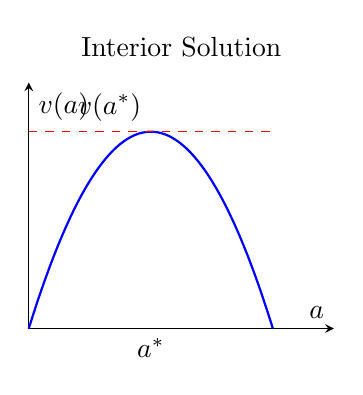
\begin{tikzpicture}
    \begin{axis}[
        width=0.45\textwidth,
        axis lines=middle,
        xlabel={$a$},
        ylabel={$v(a)$},
        xmin=0, xmax=5,
        ymin=0, ymax=5,
        xtick=\empty,
        ytick=\empty,
        domain=0:4,
        samples=100,
        title={Interior Solution},
        clip=false
    ]
        % Hemisphere-like concave function
        \addplot[thick, blue] {4 - (x - 2)^2};
        % Horizontal line through the maximum
        \addplot[dashed, red] coordinates {(0,4) (4,4)};
        \node[below] at (axis cs:2,0) {$a^*$};
        \node[left] at (axis cs:2,4.5) {$v(a^*)$};
    \end{axis}
\end{tikzpicture}
\hspace{1cm} % Add horizontal spacing between the graphs
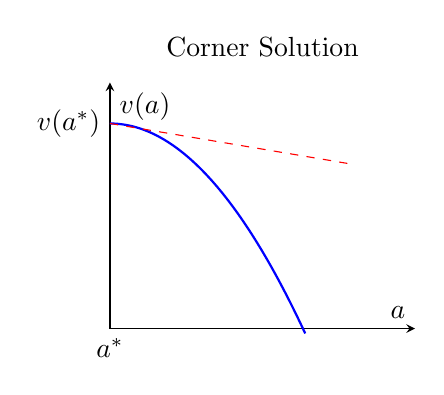
\begin{tikzpicture}
    \begin{axis}[
        width=0.45\textwidth,
        axis lines=middle,
        xlabel={$a$},
        ylabel={$v(a)$},
        xmin=0, xmax=5,
        ymin=0, ymax=6,
        xtick=\empty,
        ytick=\empty,
        domain=0:3.2,
        samples=100,
        title={Corner Solution},
        clip=false
    ]
        % Concave function starting at y=5
        \addplot[thick, blue] {5 - 0.5*x^2};
        % Line indicating the corner solution
        \addplot[dashed, red] coordinates {(0,5) (4,4)};
        \node[left] at (axis cs:0,5) {$v(a^*)$};
        \node[below] at (axis cs:0,0) {$a^*$};
    \end{axis}
\end{tikzpicture}
\end{center}

\subsection{Problem types}
\begin{enumerate}
    \item Solving for the risk premium or the certainty equivalence, with a given utility function, the probability of both outcomes, and the expected payoffs, or average payment values. 
    \item Consider an agent with a VN-M utility function \( U(w) = -e^{-w} \). He is offered a gamble that gives him wealth \( w_1 \) with probability \( p \) and wealth \( w_2 \) with probability \( 1-p \). What amount of sure wealth would make him indifferent to taking the gamble?

\end{enumerate}



%%%%%%%%%%%%% Key definitions and tables for easy review %%%%%%%%%%%%%%%%
\section{Useful takeaways}

\subsection{Axioms of preference relations}
% check proof is best fit for definition
\begin{table}[H]
    \centering
    \renewcommand{\arraystretch}{1.5}
    \setlength{\tabcolsep}{6pt} % Adjust column padding for clarity
    \begin{tabular}{|>{\centering\arraybackslash}m{2.5cm}|>{\arraybackslash}m{7cm}|>{\arraybackslash}m{7cm}|}
        \hline
        \textbf{Axiom} & \textbf{Description} & \textbf{Mathematical Proof or Logic} \\ \hline
        \textbf{Completeness} & For any two bundles \( x \) and \( y \), the consumer can rank them such that either \( x \succeq y \) (bundle \( x \) is at least as good as \( y \)) or \( y \succeq x \), or both. This ensures that the consumer has a preference between any two bundles. & The completeness axiom can be logically proven by constructing a preference relation \( \succeq \) on the set of all bundles, ensuring that for any \( x \) and \( y \), either \( x \succeq y \) or \( y \succeq x \) holds. This guarantees the existence of a complete preference ordering. \\ \hline
        \textbf{Transitivity} & For any three bundles \( x \), \( y \), and \( z \), if \( x \succeq y \) and \( y \succeq z \), then \( x \succeq z \). This property ensures consistency in preferences and is crucial for rational decision-making. & Transitivity implies consistency: if \( x \succeq y \) and \( y \succeq z \), then \( x \succeq z \). Proving this involves showing that if a preference ordering \( \succeq \) satisfies this condition, then the ordering will not cycle, ensuring rational preferences. \\ \hline
        \textbf{Continuity} & If \( x \succeq y \), then any bundle sufficiently close to \( x \) will also be preferred to or indifferent to \( y \). Formally, if \( x \succeq y \), then small changes in \( x \) will not lead to a sudden preference for \( y \). This property enables the representation of preferences with a continuous utility function. & Continuity is proven by showing that the preference relation \( \succeq \) is closed in the topological sense. If \( x_n \to x \) and \( y_n \to y \) with \( x_n \succeq y_n \) for all \( n \), then \( x \succeq y \) as \( n \to \infty \). This guarantees that small changes in \( x \) or \( y \) do not affect the preference ordering. \\ \hline
        \textbf{Local Nonsatiation and Monotonicity} & \textbf{Local Nonsatiation}: For any bundle \( x \), there exists another bundle arbitrarily close to \( x \) that is strictly preferred. This implies that more is generally better in the consumer’s immediate vicinity. & \textbf{Local Nonsatiation}: Prove that for any \( x \), for any \( \epsilon > 0 \), there exists \( y \) with \( ||y - x|| < \epsilon \) and \( y \succ x \). \\ 
        & \textbf{Monotonicity}: If \( x \) has at least as much of each good as \( y \) and more of at least one good, then \( x \succ y \). Monotonicity implies that larger quantities of goods are at least as desirable as smaller quantities.
        & \textbf{Monotonicity}: Show that for any \( x, y \) where \( x \geq y \) and \( x_i > y_i \) for some \( i \), \( x \succ y \) holds. This property is used to demonstrate that increases in any good lead to strictly preferred bundles. \\ \hline
        \textbf{Convexity} & Preferences are convex if, for any bundles \( x \) and \( y \) with \( x \sim y \), any convex combination of \( x \) and \( y \) (such as \( \lambda x + (1 - \lambda)y \) for \( \lambda \in [0,1] \)) is at least as good as \( x \) or \( y \). This implies that consumers prefer averages or balanced combinations of bundles, rather than extremes. & Convexity is shown by proving that if \( x \sim y \), then for any \( \lambda \in [0, 1] \), \( \lambda x + (1 - \lambda)y \succeq x \) and \( \lambda x + (1 - \lambda)y \succeq y \). The convexity of preferences implies that the indifference curves will be convex to the origin, ensuring a preference for diversified bundles. \\ \hline
    \end{tabular}
    \caption{Axioms of Preference and Utility}
    \label{tab:axioms_table}
\end{table}



\subsection{Theorems}
\begin{enumerate}
    \item \textbf{Roy's identity}\label{roy}: Marshallian demand for a good can be derived from the indirect utility function by comparing the impact of a change in price and a change in income, this connects indirect utility to observable demand behavior. The theorem states:
    \[
    x_i(p^0,y^0) = \frac{dv(p^0,y^0)}{dp_{i}} \Big/ \frac{dv(p^0,y^0)}{dy}
    \]
    \item \textbf{Young's Theorem}\label{YT}: Ensures the cross-partial derivatives are symmetric, which is necessary for consistency in in marginal utility, second order conditions of the cost function, and Slutsky's equation. 
    \[
    \frac{\partial^2f}{\partial x\partial y} = \frac{\partial^2f}{\partial y\partial x}
    \]
    \item \textbf{Shephard's Lemma}\label{SL}
    \[
    \frac{\partial e(p_i,u)}{\partial p_i} = h(p,u) \text{ for } i = 1,...n
    \]
    \item \textbf{Envelope Theorem}\label{ET}
    Let \( F(x, \theta) \) be a continuously differentiable function where \( x^*(\theta) \) solves:
        \[
        \max_{x} F(x, \theta).
        \]
        Then the derivative of the optimal value \( V(\theta) = F(x^*(\theta), \theta) \) with respect to the parameter \( \theta \) is given by:
        \[
        \frac{dV(\theta)}{d\theta} = \frac{\partial F(x, \theta)}{\partial \theta} \Bigg|_{x = x^*(\theta)}.
        \]
        We have multiple parameterized families of functions in which the theorem can be applied to understand the effect of changing $\alpha$ on the maximum value function, $V(\alpha)$. There is smooth dependence of the maximizers on the parameters in each problem. These include:
        \begin{itemize}
            \item \textit{Unconstrained optimization}, where we only need to consider the direct effect of $\alpha_i$ on $f(x;\alpha)$ to see the change in the value function: 
            \[
            \frac{\partial V(\alpha)}{\partial \alpha_i} = \frac{\partial f}{\partial \alpha_i}[x^*(\alpha);\alpha] \text{ for } i = 1,...I
            \] 
            \item For \textit{constrained optimization} with Lagrange:
            \[
            \frac{\partial V(\alpha)}{\partial \alpha_i} = \frac{\partial L}{\partial \alpha_i}[x^*(\alpha), \mu^*(\alpha); \alpha] \text{ for } i = 1,...I
            \]
            \item For \textit{constrained optimization} in a Kuhn-Tucker problem:
            \[
            \frac{\partial V(\alpha)}{\partial \alpha_i} = \frac{\partial L}{\partial \alpha_i}[x^*(\alpha), \lambda^*(\alpha); \alpha] \text{ for } i = 1,...I
            \]\textbf{}
        \end{itemize}
    \item \textbf{Walras' Law}\label{WL}
    states there is no excess demand. Let there be \( n \) goods in the economy, with:
    \begin{itemize}
        \item \( p = (p_1, p_2, \dots, p_n) \): The vector of prices of the goods,
        \item \( x_i^d(p) \): The demand for good \( i \) as a function of prices,
        \item \( x_i^s(p) \): The supply of good \( i \) as a function of prices.
    \end{itemize}
        Define the excess demand function for good \( i \) as:
        \[
        z_i(p) = x_i^d(p) - x_i^s(p), \quad \forall i = 1, 2, \dots, n.
        \]
    
        Walras' Law states:
        \[
        \sum_{i=1}^n p_i z_i(p) = 0.
        \]
    \item \textbf{Implicit function theorem:} Allows us to use an endogenous variable, $x$, and its dependency on an exogenous variable, $\alpha$ to define $x$ implicitly. This is useful for optimization, because the IFT provides conditions under which an equation can be expressed as a function. This ensures that small changes in \( x \) lead to predictable changes in \( y \). We can understand how solutions depend on parameters and how variables adjust to small variations. The theorem requires:
    \[
    \frac{\partial F(x, \alpha)}{\partial x} \neq 0
    \]
    Suppose $x = x(\alpha)$ is a continuously differentialble solution to the equation $F(x; \alpha) = 0$, so 
    \[
    F[x(\alpha); \alpha] = 0 \text{ then, by the Chain Rule we have}
    \]
    \[
    \frac{\partial F}{\partial \alpha}[x(\alpha^*); \alpha^*]\frac{d \alpha}{d \alpha} + \frac{\partial F}{\partial x}[x(\alpha^*); \alpha^*]\frac{dx}{d \alpha}(\alpha^*) = 0
    \]
    Solve for $\frac{d x}{d \alpha}$:
    \[
    \frac{dx}{d \alpha} = -\frac{\partial F}{\partial \alpha}[x(\alpha^*); \alpha^*]/\frac{\partial F}{\partial x}[x(\alpha^*); \alpha^*]
    \]
    So if the solution $x(\alpha)$ to $F(x;\alpha)$ exists and is continuously differentiable and $\frac{\partial F(x;\alpha)}{\partial x} \neq 0$ at the optimal value of $\alpha$, $\alpha^*$, is available, then we can solve the equation. This is a necessary and sufficient condition. The theorem gives us three statements:
    \begin{enumerate}
        \item $F[x(\alpha); \alpha] = 0$ for all $\alpha$ in $I$
        \item $x(\alpha^*) = x^*$
        \item $\frac{dx}{d \alpha}(\alpha^*) = -\frac{\partial F}{\partial \alpha}[x(\alpha^*); \alpha^*]/\frac{\partial F}{\partial x}[x(\alpha^*); \alpha^*]$
    \end{enumerate}
    \item The \textbf{Slutsky Equation} for good \( i \) is given by:
        \[
        \frac{\partial x_i^*(p, y)}{\partial p_j} = \frac{\partial h_i(p, u)}{\partial p_j} - x_i^*(p, y) \frac{\partial x_j^*(p, y)}{\partial y}.
        \]
        
        \begin{itemize}
            \item \textbf{Total Effect:} \( \frac{\partial x_i^*(p, y)}{\partial p_j} \) is the change in demand for good \( i \) due to a price change.
            \item \textbf{Substitution Effect:} \( \frac{\partial h_i(p, u)}{\partial p_j} \) is the change in demand holding utility constant.
            \item \textbf{Income Effect:} \( -x_i^*(p, y) \frac{\partial x_j^*(p, y)}{\partial y} \) is the change in demand due to the impact of the price change on real income.
        \end{itemize}
\end{enumerate}


\subsection{Comparison of utility functions}
Different utility functions have forms with different properties that can identify some clues for how it should be maximized. Below we go through common utility forms:
\begin{enumerate}

    \item \textbf{Perfect substitutes}:\label{perf} This type of utility has goods with constant rates of marginal substitution, meaning that whether you maximize, let's say $x_1$ or $x_2$ depends on the relative prices.
    \[
    u(x_1, x_2,...x_n) = min\{x_1, x_2\} + x_3 \\ 
    \text{ then either } min\{x_1, x_2\} = x_1 \text{ or } min\{x_1, x_2\} = x_2 \text{ with: } 
    \frac{p_1}{p_2} \text{ or } \frac{p_1}{p_3} \]

    So you can see that depending on the price - there is a corner solution. Let's just look at the first case:
    \begin{align}
    \text{If }  p_1 > p_2: x_1* = 0 \And x_2* = y/p_2 \\
    \text{If }  p_1 < p_2: x_1* = y/p_1 \And x_2* = 0 \\ 
    \text{If }  p_1 = p_2: x_1* = \frac{y - p_2x_2*}{p_1} \And x_2* = \frac{y - p_1x_1*}{p_2}
     \end{align}
    
    \item \textbf{Perfect complementarity (Leontif preferences):} This is when goods are consumed in certain ratios. This is the case where min\{$x_1$, $x_2$,...$x_n$\} and therefore $x_1 = x_2 = x_n$ at the optimum. To solve for this type of objective function, we set all bundles of good equal to each other, solving for one bundle, let's say $x_2$. Then, substitute $x_2$ into the budget constraint to get $x_1*$. 
    \begin{align}
    \text{ a simple case: } u(x_1, x_2) = \min \{ ax_1, bx_2 \} \\ 
    \text{ a more complex case: } u(x_1, \ldots, x_n) = (ax_1 + b \min \{x_2, \ldots, x_n\})^2
    \end{align}
    Where in the more complex case, we assume $M$ is some amount of money spent on the goods in the minimization bundle, and therefore the first order conditions are: 
    \[
    \Tilde{x} = \frac{M}{\sum_{i=2}^{n} p_i} \text{  and  } x_1 = \frac{y-M}{p_1} 
    \]
    Where Walrasian demand functions need to be solved for the cases where the price ratios (or $\Tilde{x}$ and $x_1$) are greater than, less than or equal. 
    \item \textbf{Constant elasticity of substitution (CES):} This is a case where the utility is continuous and increasing in the goods, $x_i$ by the properties of the utility function. Perfect substitutes\ref{perf} are a special case of CES. An example of CES, generally (in LaGrange form) is:
    \begin{align}
        L(x_1,x_2,p_1,p_2) = (x^p_1 + x^p_2)^{1/p} - \lambda (p_1x_1 + p_2x_2 - y)
    \end{align}
    \item \textbf{Lexicographic preferences:}\label{lex} A strict ranking of goods where a consumer always prioritizes one good over another, regardless of quantity. The consumer never trades a higher-priority good for any amount of a lower-priority good. This form of preferences \textit{violate continuity}, making them incompatible with standard utility representations. 
    
    A preference relation \( \succ \) on \( \mathbb{R}^n_+ \) is \textbf{lexicographic} if for any two bundles \( x = (x_1, x_2, \dots, x_n) \) and \( y = (y_1, y_2, \dots, y_n) \):

    \begin{align}
        x \succ y \quad \text{if and only if} \quad \exists \, k \in \{1, \dots, n\} \text{ such that } x_k > y_k \text{ and } x_j = y_j \text{ for all } j < k.
    \end{align}

\end{enumerate} 



\subsection{Comparison of demand functions}
\begin{table}[H]
    \centering
    \renewcommand{\arraystretch}{1.3}
    \setlength{\tabcolsep}{5pt} % Adjust column padding
    \resizebox{0.95\textwidth}{!}{ % Resize table to 90% of text width
    \begin{tabular}{|>{\centering\arraybackslash}m{3.5cm}|>{\centering\arraybackslash}m{4cm}|>{\centering\arraybackslash}m{3.5cm}|>{\centering\arraybackslash}m{3.5cm}|>{\centering\arraybackslash}m{4cm}|}
        \hline
        \textbf{Function} & \textbf{Form} & \textbf{Homogeneity} & \textbf{Increasing/ Decreasing} & \textbf{Concavity/Convexity} \\ \hline
        \textbf{Direct (Walrasian) Demand} & \( x_i(p, w) = \frac{\alpha_i w}{p_i} \) (for Cobb-Douglas) & Degree 0 in \( p \) and \( w \) & Increasing in \( w \), decreasing in \( p \) & Quasiconvex in \( p \); convex in \( w \) \\ \hline
        \textbf{Indirect Utility Function} & \( v(p, w) = u(x_1(p, w), \dots, x_n(p, w)) \) & Degree 0 in \( p \) and \( w \) & Increasing in \( w \), decreasing in \( p \) & Quasiconcave in \( w \); quasiconvex in \( p \) \\ \hline
        \textbf{Expenditure Function} & \( e(p, u) = \min_{x} \{ p \cdot x : u(x) = u \} \) & Degree 1 in \( p \), degree 1 in \( u \) & Increasing in \( u \), increasing in \( p \) & Concave in \( p \); linear in \( u \) \\ \hline
        \textbf{Compensated (Hicksian) Demand} & \parbox{3.5cm}{\( h_i(p, u) = \frac{\partial e(p, u)}{\partial p_i} \) \\ (Cobb-Douglas: \( h_i(p, u) = \frac{\alpha_i u}{p_i} \))} & Degree 0 in \( p \) and \( u \) & Increasing in \( u \), decreasing in \( p \) & Concave in \( p \); convex in \( u \) \\ \hline
    \end{tabular}
    }
    \caption{Properties of Key Functions in Consumer Theory}
    \label{tab:consumer_functions}
\end{table}



\subsection{Duality}
% table summarizing the dual relationships$
\renewcommand{\arraystretch}{1}
    \begin{longtable}{|>{\raggedright\vspace{-0.75em}\arraybackslash}p{2cm}|>{\centering\vspace{-0.75em}\arraybackslash}p{5cm}|>{\raggedright\vspace{-.75em}\arraybackslash}p{8cm}|}
    \hline
    \textbf{Relation} & \textbf{Expression} & \textbf{Properties} \\ \hline
    Direct $\Leftrightarrow$ indirect utility &
    \[
    V(p, y) = U(x^*(p, y))
    \] &
    \begin{itemize}\setlength{\itemsep}{-.5em}
        \item Indirect utility maximizes $U(x)$ under budget constraints
        \item Homogeneity of degree 0 in $(p, y)$
        \item Quasiconvex in prices
    \end{itemize} \\ \hline
    
    Indirect utility $\Leftrightarrow$ expenditure  &
    \[
    V(p, y) = U \Leftrightarrow E(p, U) = y
    \] &
    \begin{itemize}\setlength{\itemsep}{-.5em}
        \item Expenditure minimizes cost for a target utility level
        \item Duality: $V(p, y) \Leftrightarrow E(p, U)$
        \item Expenditure is concave in prices
    \end{itemize} \\ \hline
    
    Expenditure $\Leftrightarrow$ Hicksian demand &
    \[
    E(p, U) = \sum p_i \cdot h_i(p, U)
    \] &
    \begin{itemize}\setlength{\itemsep}{-.5em}
        \item Hicksian demand minimizes expenditure for target utility
        \item Derived from Shephard's Lemma
        \item Homogeneous of degree 0 in prices
    \end{itemize} \\ \hline
    
    Indirect utility $\Leftrightarrow$ Marshallian demand &
    \[
    x_i^*(p, y) = -\frac{\partial V(p, y)}{\partial p_i} \div \frac{\partial V(p, y)}{\partial y}
    \] &
    \begin{itemize}\setlength{\itemsep}{-.5em}
        \item Roy’s Identity links demand and indirect utility
        \item Indirect utility is differentiable in $p$ and $y$
        \item Homogeneous of degree 0 in $(p, y)$
    \end{itemize} \\ \hline
    
    Marshallian $\Leftrightarrow$ Hicksian demand &
    \[
    h_i(p, U) = x_i^*(p, E(p, U))
    \] &
    \begin{itemize}\setlength{\itemsep}{-.5em}
        \item Hicksian adjusts for utility changes; Marshallian adjusts for income changes
        \item Linked via $E(p, U)$
    \end{itemize} \\ \hline
    \caption{Duality relationships}
    \label{tab:duality_table}
\end{longtable}


\end{document}


